\documentclass[man, noextraspace, floatsintext]{apa6}\usepackage[]{graphicx}\usepackage[]{color}
%% maxwidth is the original width if it is less than linewidth
%% otherwise use linewidth (to make sure the graphics do not exceed the margin)
\makeatletter
\def\maxwidth{ %
  \ifdim\Gin@nat@width>\linewidth
    \linewidth
  \else
    \Gin@nat@width
  \fi
}
\makeatother

\definecolor{fgcolor}{rgb}{0.345, 0.345, 0.345}
\newcommand{\hlnum}[1]{\textcolor[rgb]{0.686,0.059,0.569}{#1}}%
\newcommand{\hlstr}[1]{\textcolor[rgb]{0.192,0.494,0.8}{#1}}%
\newcommand{\hlcom}[1]{\textcolor[rgb]{0.678,0.584,0.686}{\textit{#1}}}%
\newcommand{\hlopt}[1]{\textcolor[rgb]{0,0,0}{#1}}%
\newcommand{\hlstd}[1]{\textcolor[rgb]{0.345,0.345,0.345}{#1}}%
\newcommand{\hlkwa}[1]{\textcolor[rgb]{0.161,0.373,0.58}{\textbf{#1}}}%
\newcommand{\hlkwb}[1]{\textcolor[rgb]{0.69,0.353,0.396}{#1}}%
\newcommand{\hlkwc}[1]{\textcolor[rgb]{0.333,0.667,0.333}{#1}}%
\newcommand{\hlkwd}[1]{\textcolor[rgb]{0.737,0.353,0.396}{\textbf{#1}}}%

\usepackage{framed}
\makeatletter
\newenvironment{kframe}{%
 \def\at@end@of@kframe{}%
 \ifinner\ifhmode%
  \def\at@end@of@kframe{\end{minipage}}%
  \begin{minipage}{\columnwidth}%
 \fi\fi%
 \def\FrameCommand##1{\hskip\@totalleftmargin \hskip-\fboxsep
 \colorbox{shadecolor}{##1}\hskip-\fboxsep
     % There is no \\@totalrightmargin, so:
     \hskip-\linewidth \hskip-\@totalleftmargin \hskip\columnwidth}%
 \MakeFramed {\advance\hsize-\width
   \@totalleftmargin\z@ \linewidth\hsize
   \@setminipage}}%
 {\par\unskip\endMakeFramed%
 \at@end@of@kframe}
\makeatother

\definecolor{shadecolor}{rgb}{.97, .97, .97}
\definecolor{messagecolor}{rgb}{0, 0, 0}
\definecolor{warningcolor}{rgb}{1, 0, 1}
\definecolor{errorcolor}{rgb}{1, 0, 0}
\newenvironment{knitrout}{}{} % an empty environment to be redefined in TeX

\usepackage{alltt}
\newcommand{\bibfile}{C:/Users/jep2963/Documents/Bibliography/Behavioral_observation-APP}  

\usepackage[natbibapa]{apacite}
\newcommand{\citetal}[1]{\shortcites{#1}\citet{#1}}

\raggedbottom

\usepackage{amssymb}
\usepackage{amsmath}
\usepackage{amsthm}
\newtheorem{lemma}{Lemma}

\usepackage{graphicx}

\usepackage{fixltx2e}
\usepackage{subcaption}
\usepackage{float}

\usepackage{array}
\usepackage{multirow}
\usepackage{rotating}
\setlength{\rotFPtop}{0pt plus 1fil}
\usepackage[draft]{changes}

\geometry{twoside=false, top=1in, bottom=1in, left=1in, right=1.2in}
\usepackage[textwidth=1in, textsize=tiny]{todonotes}

\newcommand{\Prob}{\text{Pr}}
\newcommand{\E}{\text{E}}
\newcommand{\Cov}{\text{Cov}}
\newcommand{\corr}{\text{corr}}
\newcommand{\Var}{\text{Var}}
\newcommand{\iid}{\stackrel{\text{iid}}{\sim}}
\newcommand{\logit}{\text{logit}}
\newcommand{\cll}{\text{cll}}


\title{Estimating the prevalence and incidence of a state behavior: Models for interval recording data and a novel observation system}
\shorttitle{ESTIMATING PARAMETERS OF A STATE BEHAVIOR}
\twoauthors{James E. Pustejovsky and Daniel M. Swan}{Austin H. Johnson}
\twoaffiliations{The University of Texas at Austin}{University of Connecticut}
\leftheader{Pustejovsky, Swan, & Johnson}
 
\abstract{Data based on direct observation of behavior are used widely in many areas of educational and psychological research, particularly in applied research areas such as the treatment of behavioral disorders. 
A number of different methods are used to record data during direct observation, including continuous recording, momentary time sampling (MTS), partial interval recording (PIR), and whole interval recording (WIR). 
Among these methods, PIR and WIR have long been recognized as problematic because, as typically reported, the mean of such data measures neither the prevalence nor the incidence of the observed behavior. 
Though the problems with these methods have long been recognized, little research has examined methods of analyzing interval recording data other than simply taking the mean. 
This paper proposes a Alternating Poisson Process model for interval recording data that permits estimation of both prevalence and incidence via maximum likelihood or penalized maximum likelihood methods. 
The paper also describes a novel observation recording method that involve combinations of MTS, PIR, and WIR and that provides considerably more efficient estimators of prevalence and incidence.}

\keywords{behavioral observation; interval recording; alternating Poisson process; Markov chain}

\authornote{James E. Pustejovsky, Department of Educational Psychology, University of Texas at Austin. Daniel M. Swan, Department of Educational Psychology, University of Texas at Austin. Austin H. Johnson, Department of Educational Psychology, University of Connecticut. 

Address correspondence to James E. Pustejovsky, Department of Educational Psychology, University of Texas at Austin, 1 University Station D5800, Austin, TX 78712. Email: pusto@austin.utexas.edu.}
\IfFileExists{upquote.sty}{\usepackage{upquote}}{}
\begin{document}


\maketitle

Measurements derived from systematic, direct observation of human behavior are used in many areas of psychological and educational research. 
For example, direct observation of student classroom behavior is a primary component of several existing instruments for screening and diagnosis of emotional and behavioral problems \citep{Volpe2005observing}; direct observation of childrens' challenging behavior in home settings has been employed to collect pre- and post-test measures in randomized trials of behavioral interventions \citep[e.g.,][]{Durand2012positive}; and direct observation of infant-parent interaction patterns is employed in studies of child development \citep{Mann1991time} and cross-cultural differences \citep{Bornstein2002measurement}. 
Direct observation also plays a prominent role in single-case research, where it is used to assess individual responses to intervention by measuring changes in behavior over time \citep{Kazdin2011single}.

Systematic direct observation procedures require that the behavior of interest have a clear operational definition, so that its occurrence or absence can be judged at a given point in time. 
In forming such an operationally definition, is useful to distinguish between behaviors that are events, where each occurrence is of negligible duration, versus behaviors that are states, where individual episodes of behavior have positive duration \citep{Altmann1974observational}. 
The primary characteristic of an event behavior is its incidence, or frequency of occurrence per time unit. 
In contrast, a state behavior has two primary characteristics: incidence, which is the frequency (per unit time) with which new episodes of the behavior begin and prevalence, which is the proportion of time that the behavior occurs. Given an operationally defined behavior, measurements of its characteristics are obtained by recording data while observing the behavior (either in person, or by video-recording) for a specified length of time. 

There are several different procedures for recording data during direct observation, varying in ease of implementation, the level of detail in the resulting data, and the aspect of behavior to which the resulting measurement corresponds \citep[for surveys of major recording procedures, see][]{Altmann1974observational, Ayres2010dependent, Hartmann1990observational, Primavera1996measurement}. 
The most intensive procedure is continuous recording (sometimes called duration recording or real-time recording), in which the observer records the time at which each behavioral episode begins and ends.
Data from continuous recording is very rich, in that it permits direct estimation of prevalence, incidence, and further aspects of the pattern of behavior; continuous recording data can also be subjected to more sophisticated forms of modeling \citep[e.g.,][]{Bakeman2011sequential, Haccou1992statistical}. 
However, less effort-intensive data collection methods are often required, particularly for use in clinical and applied research settings. 

Other commonly used systems for collecting behavioral data do not capture a complete record of the behavior during an observation session, but rather involve making observations only intermittently. 
Among intermittent recording systems, the three main procedures are momentary time sampling, partial interval recording, and whole interval recording. 
In all three methods, an observation session is divided into a fixed number of equally spaced intervals, of perhaps 10 or 15 s in length, and a binary data-point is recorded for each interval. 
The systems differ only in the rule for scoring each interval. 
Using momentary time sampling (MTS), an interval is scored as a one if a behavioral event is happening during the final moment of the interval (and is otherwise scored as a zero). 
Using partial interval recording (PIR, also known as one-zero sampling, modified frequency sampling, or Hansen sampling), an interval is scored as a one if the behavior occurs at any point during the interval. 
Using whole interval recording (WIR), an interval is scored as a one only if the behavior occurs for the entire duration of the interval. 
In some PIR and WIR systems, a small length of time is left between each interval so that the observer does not have to maintain continuous attention. 

In many applications, the interval-by-interval data generated by these recording systems is summarized by the proportion of intervals scored as a one. 
Often, only this summary proportion is used for later analysis, where it is interpretted as a measure of prevalence. 
However, whether it is reasonable to reduce the data to a summary proportion depends on which recording system is used to collect the data. 

Under quite general modeling assumptions, the proportion of MTS intervals is an unbiased estimate of prevalence \citep{Rogosa1991statistical}. 
Thus, reducing the data to the summary proportion is entirely reasonable if the investigator's interest is solely in the prevalence of the behavior. 
The drawback of doing so is that simple summaries of MTS data do not provide any measure of the behavior's incidence. 
Even if not of substantive interest, an estimates of incidence is needed in order to assess the magnitude of measurement error in the prevalence estimate. 

\citet[see also \citealp{Griffin1983parametric}]{Brown1977estimation} described a method for estimating both prevalence and incidence from MTS data. 
Their approach was to first posit a stochastic process for the underlying pattern of behavior as perceived by the observer, or what is often termed the behavior stream. 
The particular model they considered was an Alternating Poisson Process, which is a simple, two-state continuous time Markov chain where transitions between states follow exponential distributions. 
Brown and colleagues showed that if the behavior stream is generated by such a process, then interval-by-interval MTS scores follow a discrete-time Markov chain, from which closed-form expressions for the maximum likelihood estimators of prevalence and incidence can be derived.

Unlike MTS, PIR and WIR systems do not produce clearly interpretable summary measurements. 
Rather, the PIR summary proportion systematically over-estimates prevalence and the WIR summary proportion systematically under-estimates prevalence; in both cases, the extent of the bias depends on characteristics of the behavior as well as operational features of the recording system \citep{Kraemer1979one, Rogosa1991statistical}, making the construct interpretation of such data quite difficult. 
Consequently, methodologists have long argued against the use of PIR and WIR systems \citep[cf.]{Altmann1974observational, Mann1991time, Lane2014using}. 
Despite such objections, the systems remain in common use, particularly as part of behavioral time series designs and single-case research \citep{Rapp2007interval, Mudford2009continuous, Lane2014using}. 

Little previous research has considered methods of analyzing PIR and WIR data beyond using the summary proportion.
For PIR data, \citet{Altmann1970estimating} proposed a transformation of the summary proportion as an estimate of incidence, motivated by a model in which behavioral episodes follow a Poisson process. While this model applies well to event behaviors, it is not a suitable description of state behaviors, where individual episodes have non-negligible duration. 
\citet{Suen1986post, Suen1989analyzing} have proposed a method for obtaining estimates of prevalence and incidence from PIR data, provided that the behavior stream conforms to certain conditions. 
However, their proposed procedure is not motivated by any explicit data-generating process, and later simulation studies reported that the method produces badly biased estimates \citep[sec. 5.2]{Rogosa1991statistical}. 
\citet{Pustejovsky2014four} proposed several methods for bounding the bias of the PIR summary proportion as an estimate of prevalence, based on various prior assumptions about the behavior stream. 
These methods are useful for analysis of summarized PIR data, as would be available from a published single-case study, but are not full models of the data-generating process.
Other methods of analysis, involving fully specified data-generating models for the interval-by-interval scores, are therefore of interest.

This paper examines models for PIR and WIR data, from which principled estimates of prevalence and incidence can be obtained. 
Following \citet{Brown1977estimation}, we use an Alternating Poisson Process for the underlying behavior stream to derive a model for the interval-by-interval scores. 
Under this model, maximum likelihood estimates for prevalence and incidence can be obtained using conventional numerical techniques (although they do not have closed-form expression). 
To remedy some problems with the maximum likelihood estimators, we introduce penalized likelihood estimators that have better operating characteristics and that can be tailored to express prior information about the behavioral parameters.
\todo{We use a parametric bootstrap procedure for obtaining interval estimates.} 
The final section of the paper describes a novel procedure for intermittent recording of a behavior that entails combining MTS and interval recording methods and that can be used to obtain more efficient estimators of prevalence and incidence.

\section{Alternating Poisson Process models}
\label{sec:APP}

The Alternating Poisson Process is a stochastic model that can be used to describe a stream of behavior, as it is perceived in time. 
The model applies to state behaviors, where the behavior is either occurring or not occurring at any given point in time and where each episode of behavior has non-negligible duration. 
The stream of a state behavior can be described in terms of two components: sequentially ordered, non-overlapping episodes of behavior, which we will call event durations, and spans of time in between episodes, which we will call interim times. 
Let $\{Z(t), 0 \leq t\}$ denote the state of the behavior stream over the course of an observation session, where $Z(t) = 1$ indicates that an event is occurring at time $t$ and $Z(t) = 0$ otherwise.

The Alternating Poisson Process makes several further assumptions. 
Specifically, it is assumed that event durations and interim times are mutually independent, random quantities, that the event durations follow an exponential distribution with mean $\mu > 0$, and that the interim times follow an exponential distribution with mean $\lambda > 0$. 
Under the model, the prevalence of the behavior is equal to the ratio of $\mu$ to the sum of $\mu$ and $\lambda$ and the incidence of the behavior is equal to the reciprocal of the sum of $\mu$ and $\lambda$. 
We will denote prevalence by $\phi$, where $0 < \phi < 1$, and incidence by $\zeta$, where $\zeta > 0$. Finally, it is assumed that the process is in equilibrium, with $\Pr\left(Y(0) = 1\right) = \phi$. 
This assumption implies that there is a constant marginal probability of observing an event at any given point in time.

The Alternating Poisson Process is a special case of a continuous time Markov chain, and thus has the Markov property that the future evolution of the behavior depends only on the current state, but not on the past history of the behavior. 
More precisely, the probability that a behavior will be occurring $t$ seconds into the future is independent of the state of the behavior for $0 \leq r < s$: 
\begin{equation}
\label{eq:Markov}
\Pr\left[Z(s + t) = 1 \left| Z(s) = a, Z(r): 0 \leq r < s \right.\right] = \Pr\left[ Z(s + t) = 1 \left| Z(s) = a \right.\right]
\end{equation}
for $a = 0,1$ and $s,t \geq 0$ \citep[Thm. 6.1]{Kulkarni2010modeling}. 
The assumption that the process is in equilibrium further implies that the probability that a behavior will be occurring $t$ seconds into the future does not depend on the current time, i.e.,  
\begin{equation}
\label{eq:equilibrium}
\Pr\left[Z(s + t) = 1 \left| Z(s) = a\right.\right] = \Pr\left[ Z(t) = 1 \left| Z(0) = a \right.\right].
\end{equation}
Let $p_a(t)$ denote the conditional probability that an event will be occurring $t$ seconds into the future, given that the behavior is currently in state $a$, for $a = 0,1$. 
These conditional probabilities can be expressed as follows:
\begin{equation}
\begin{aligned}
p_0(t) &= \Pr(Z(t) = 1 | Z(0) = 0) = \phi \left[1 - \exp\left(\frac{- t \zeta}{\phi (1 - \phi)}\right)\right] \\
p_1(t) &= \Pr(Z(t) = 1 | Z(0) = 1) = \phi + (1 - \phi) \exp\left(\frac{- t \zeta}{\phi (1 - \phi)}\right)
\end{aligned}
\end{equation}
\citep[Eq. 6.17]{Kulkarni2010modeling}.

\subsection{Momentary Time Sampling}
\label{subsec:MTS}

Consider observing a behavior stream generated by the Alternating Poisson Process and recording observations using momentary time sampling with $K + 1$ recording times, equally spaced at intervals of length $c$. 
Denote the recorded data by the sequence of binary indicator variables $X_0,X_1,...,X_K$. The MTS interval data are a record of the state of the behavior stream process at fixed moments in time: $X_k = Z(ck)$ for $k = 0,...,K$. 

\citet{Brown1977estimation} demonstrated that MTS data follow a two-state, discrete-time Markov chain process with transition probabilities $Pr(X_k = 1 | X_{k-1} = a) = p_a(c)$ and $Pr(X_k = 0 | X_{k-1} = a) = 1 - p_a(c)$ for $a = 0,1$. 
Therefore, sufficient statistics for the process are given by the table counting the number of transitions with $(X_{k-1} = a, X_k = b)$ for $a,b = 0,1$ and $k = 1,...,K$; let $n_{ab} = \sum_{k=1}^K I(X_{k-1} = a, X_k = b)$. 
Conditioning on $X_0$, the log-likelihood of MTS data is then given by \begin{equation}
\begin{aligned}
\label{eq:MTS_loglik}
l_{MTS}(\phi, \zeta) &= n_{01} \log \phi + n_{10} \log\left(1 - \phi\right) \\
& \qquad \qquad + \left(n_{01} + n_{10}\right) \log \left[1 - \exp\left(\frac{-\zeta c}{\phi (1 - \phi)}\right)\right] \\
& \qquad \qquad \qquad \qquad + n_{00} \log\left[1 - \phi + \phi \exp\left(\frac{-\zeta c}{\phi (1 - \phi)}\right)\right]\\
& \qquad \qquad \qquad \qquad \qquad \qquad + n_{11}\log\left[\phi + \left(1 - \phi\right)\exp\left(\frac{-\zeta c}{\phi (1 - \phi)}\right)\right].
\end{aligned}
\end{equation}
\citet{Brown1977estimation} provided closed-form expressions for the maximum likelihood estimates (MLEs) for $\phi$ and $\zeta$ based on this model. Let $\hat{p}_0 = n_{01}/ \left(n_{00} + n_{01}\right)$ and $\hat{p}_1 = n_{11} / \left(n_{10} + n_{11}\right)$. The MLE for $\zeta$ exists only when $\hat{p}_0 < \hat{p}_1$. 
When this condition holds, the MLEs for $\phi$ and $\zeta$ are given by 
\begin{equation}
\label{eq:MTS_mle}
\hat\phi_{MTS} = \frac{\hat{p}_0}{\hat{p}_0 + 1 - \hat{p}_1} \qquad \text{and} \qquad
\hat\zeta_{MTS} = \frac{-\hat{p}_0 \left(1 - \hat{p}_1\right) \log(\hat{p}_1 - \hat{p}_0)}{c \left(\hat{p}_0 + 1 - \hat{p}_1\right)^2}.
\end{equation}



% latex table generated in R 3.1.2 by xtable 1.7-3 package
% Thu Mar 19 13:52:58 2015
\begin{table}[b]
\centering
\caption{Proportion of 2000 simulated MTS samples (K = 40) in which $0 < \hat\phi_{MTS} < 1$ and $0 < \hat\zeta_{MTS} < \infty$.} 
\label{tab:MTS_zeta_valid}
\begin{tabular}{rrrrrrrr}
  \hline
 & $\zeta = 0.02$ & 0.05 & 0.1 & 0.2 & 0.25 & 0.4 & 0.5 \\ 
  \hline
$\phi = 0.1$ & 0.43 & 0.63 & 0.64 & 0.45 & 0.37 & 0.29 & 0.26 \\ 
  0.2 & 0.45 & 0.80 & 0.90 & 0.84 & 0.79 & 0.59 & 0.49 \\ 
  0.3 & 0.46 & 0.84 & 0.96 & 0.96 & 0.94 & 0.73 & 0.64 \\ 
  0.4 & 0.43 & 0.87 & 0.98 & 0.99 & 0.97 & 0.82 & 0.71 \\ 
  0.5 & 0.45 & 0.88 & 0.99 & 1.00 & 0.98 & 0.84 & 0.71 \\ 
   \hline
\end{tabular}
\end{table}


The probability that the MLEs are undefined or fall outside of the parameter space is not trivial, even when $K$ is relatively large. 
In order for the estimates to fall strictly within the parameter space, both a 0-1 transition and a 1-0 transition must be observed, so that $\hat{p}_0 > 0$, $\hat{p}_1 < 1$. Table \ref{tab:MTS_zeta_valid} reports the proportion of 2000 simulated samples in which $0 < \hat\phi_{MTS} < 1$ and $0 < \hat\zeta_{MTS} < \infty$, with $K = 40$ and $\zeta$ scaled in terms of the interval length. 
Values of $\phi > 0.5$ are omitted because the behavior of the MTS estimators is symmetric about $\phi = 0.5$. 
The proportion of estimates falling within the parameter space decreases as prevalence becomes more extreme and as incidence becomes very infrequent or very frequent. 
The high proportion of samples in which the estimate of incidence is undefined represents a drawback to the use of maximum likelihood based on MTS data.

\subsection{Partial Interval Recording}
\label{subsec:PIR}

Consider observing a behavior stream generated by the Alternating Poisson Process and recording observations using partial interval recording. 
Suppose that one observes $K$ intervals, where each interval includes $c$ seconds of active observation time followed by $d$ seconds of recording time. 
Let time $t_k = (k-1)(c + d)$ denote the beginning of interval $k$. Let $U_k$ indicate the PIR score from interval $k$, corresponding to the time from $t_k$ to $t_k + c$. 
Following the PIR system, $U_k = 1$ if is the behavior occurs at any point during the active portion of interval, and $U_k = 0$ otherwise. 
In terms of the behavior stream process, 
\begin{equation}
U_k = I\left[ 0 < \int_0^c Z\left(t_k + s \right) ds\right]
\end{equation}
for $k = 1,...,K$, where $\int_0^c$ denote the definite integral over the half-open interval $[0,c)$.

Under the assumptions of the Alternating Poisson Process, the joint distribution of $U_1,...,U_K$ can be derived as follows. 
Let $\psi_k, k = 2,...,K$ denote the probability than the behavior is occurring at time $t_k = (k-1)(c + d)$, given the partial interval record up to that time. 
Let $\psi_1 = \phi$, which follows from the assumption that the process is in equilibrium. We show in Appendix \ref{app:PIR_derivation} that  
\begin{equation}
\label{eq:psi_k}
\begin{aligned}
\psi_k &= \Pr\left[ Z(t_k) = 1 \left| U_1,...,U_{k-1}\right.\right] \\
 &= \left[\frac{\psi_{k-1} p_1(c + d) + (1 - \psi_{k-1}) \left[p_0(c + d) - p_0(d) \exp\left(\frac{- \zeta c}{1 - \phi}\right)\right]}{1 - (1 - \psi_{k-1})\exp\left( \frac{-\zeta c}{1 - \phi}\right)}\right]^{u_{k-1}} \left[p_0(d)\right]^{(1 - u_{k-1})}.
\end{aligned}
\end{equation}
Note that $Z(t_k) = 1$ implies that $U_k = 1$ with certainty, while 
\[ \Pr\left(U_k = 1\left| Z(t_k) = 0\right.\right) = 1 - \exp\left( \frac{-\zeta c}{1 - \phi}\right).\]
It follows from the Markov property of the Alternating Poisson Process that 
\begin{align*}
\Pr\left(U_k = 1 \left| U_1,...,U_{k-1}\right.\right) &= \psi_k \Pr\left(U_k = 1 \left| Y(t_k) = 1)\right.\right)  + (1 - \psi_k)\Pr\left(U_k = 1 \left| Y(t_k) = 0)\right.\right) \\
&= 1 - (1 - \psi_k)\exp\left( \frac{-\zeta c}{1 - \phi}\right).
\end{align*}
The joint distribution of $U_1,...,U_K$ can therefore be expressed as 
\begin{align*}
\Pr\left(U_1=u_1,...,U_K = u_K\right) &= \Pr\left(U_1=u_1\right) \prod_{k=2}^K \Pr\left(U_k=u_k \left| U_1,...,U_{k-1}\right.\right) \nonumber \\
&= \prod_{k=1}^K \left[1 - (1 - \psi_k)\exp\left( \frac{-\zeta c}{1 - \phi}\right) \right]^{u_k} \left[(1 - \psi_k)\exp\left( \frac{-\zeta c}{1 - \phi}\right)\right]^{(1 - u_k)}.
\end{align*}

The log-likelihood of $\phi$ and $\zeta$, given observed PIR data $u_1,...,u_K$, is
\begin{align}
\label{eq:PIR_loglik}
l_{PIR}\left(\phi,\zeta\right) = \sum_{k=1}^K & u_k \ln\left[1 - (1 - \psi_k)\exp\left( \frac{-\zeta c}{1 - \phi}\right)\right]  + (1 - u_k)\left[\ln\left(1 - \psi_k \right) - \frac{\zeta c}{1 - \phi}\right].
\end{align}
MLEs $\hat\phi_{PIR}, \hat\zeta_{PIR}$ are obtained by maximizing $l_{PIR}$ using numerical techniques. 
Because the conditional probabilities $\psi_1,...,\psi_K$ are defined recursively, it is cumbersome and computationally expensive to evaluate the score function corresponding to this likelihood. 
The simulation study reported in a section therefore uses the Nelder-Mead algorithm \citep{Nelder1965simplex}, which does not require evaluation of the score function.



% latex table generated in R 3.1.2 by xtable 1.7-3 package
% Thu Mar 19 13:52:58 2015
\begin{table}[b]
\centering
\caption{Proportion of 2000 simulated PIR samples (K = 40) in which  $|\text{logit}(\hat\phi_{PIR})| < 8$ and $|\text{log}(\hat\zeta_{PIR})| < 8$.} 
\label{tab:PIR_ests_valid}
\begin{tabular}{rrrrrrrr}
  \hline
 & $\zeta = 0.02$ & 0.05 & 0.1 & 0.2 & 0.25 & 0.4 & 0.5 \\ 
  \hline
$\phi = 0.1$ & 0.59 & 0.83 & 0.94 & 0.94 & 0.90 & 0.78 & 0.72 \\ 
  0.2 & 0.67 & 0.91 & 0.98 & 0.99 & 0.98 & 0.92 & 0.84 \\ 
  0.3 & 0.74 & 0.94 & 0.99 & 1.00 & 1.00 & 0.94 & 0.87 \\ 
  0.4 & 0.78 & 0.96 & 1.00 & 1.00 & 0.99 & 0.93 & 0.86 \\ 
  0.5 & 0.77 & 0.96 & 0.99 & 0.99 & 0.98 & 0.89 & 0.80 \\ 
  0.6 & 0.75 & 0.94 & 0.97 & 0.96 & 0.92 & 0.79 & 0.67 \\ 
  0.7 & 0.68 & 0.87 & 0.92 & 0.85 & 0.78 & 0.56 & 0.38 \\ 
  0.8 & 0.60 & 0.76 & 0.77 & 0.56 & 0.42 & 0.16 & 0.09 \\ 
  0.9 & 0.47 & 0.48 & 0.32 & 0.08 & 0.04 & 0.00 & 0.00 \\ 
   \hline
\end{tabular}
\end{table}


Just as with MTS data, MLEs based on PIR data do not always fall within the parameter space. 
Table \ref{tab:PIR_ests_valid} reports the proportion of 2000 simulated samples in which the MLEs based on PIR data are within the parameter space, with $K = 40$, $d = 0$, and $\zeta$ scaled in terms of the interval length.
Because we use numerical maximization, the results of the maximization routine are never precisely on the borders of the parameter space. 
We therefore use boundaries of $|\logit \ \hat\phi_{PIR}| < 8$ and $|\log \hat\zeta_{PIR}| < 8$ to define the edges of the parameter space. 
The proportion of estimates falling within the parameter space is highest for moderate values of prevalence and incidence ($0.2 \leq \phi \leq 0.5$ and $0.1 \leq \zeta \leq 0.25$), decreases as prevalence becomes more extreme, and decreases as incidence becomes either less frequent (less than once per ten intervals) or more frequent (more than once per four intervals).  
Unlike the MTS estimators, the pattern of boundary estimates is asymmetric because PIR tends to reach ceiling levels when prevalence is large. 

In addition to returing estimates that are on the edges of the parameter space, the MLEs based on PIR data have the further disadvantage of being somewhat sensitive to initialization values. 
The likelihood surface becomes very flat when the PIR scores are near ceiling or floor levels, making it difficult to numerically identify the maximum. 
For the implementation of the estimators in the accompanying R package, the consequence is that drastically different estimates can be returned depending on the initialization values of the algorithm. 
Together with the possibility of obtaining estimates on the edges of the parameter space, the numerical instability of the MLEs motivates our investigation of alternative estimators that incorporate penalty functions.  

\subsection{Whole Interval Recording}
\label{sec:WIR}

Consider observing a behavior stream generated by the Alternating Poisson Process and recording observations using whole interval recording. 
As with PIR, suppose that one observes $K$ intervals, where each interval includes $c$ seconds of active observation time followed by $d$ seconds of recording time. 
Let $W_k$ indicate the WIR score from interval $k$, corresponding to the time from $t_k$ to $t_k + c$. 
Following the WIR system, $W_k = 1$ if is the behavior occurs for the duration of the active portion of interval, and $W_k = 0$ otherwise. 
Formally, 
\begin{equation}
W_k = I\left[ c = \int_0^c Z\left(t_k + s \right) ds\right]
\end{equation}
for $k = 1,...,K$. 

Using the WIR system to score a state behavior is logically equivalent to using PIR to score the absence of the behavior. 
WIR data can therefore be modeled just as PIR data, after an appropriate change of parameters. 
Specifically, the log-likelihood for WIR data under the Alternating Poisson Process can be written in terms of the log-likelihood for PIR data as
\begin{equation}
l_{WIR}\left(\phi, \zeta | W_1 = w_1,...,W_k = w_k \left) = l_{PIR}\right(1 - \phi, \zeta | U_1 = 1 - w_1,...,U_K = 1 - w_k\right).
\end{equation}
The equivalence of the two system implies that estimates of prevalence and incidence based on WIR data can be obtained using the algorithms developed for PIR. 


\subsection{Augmented interval recording}
\label{subsec:AIR}

Thus far, we have considered conventional and widely used procedures for intermittent, systematic direct observation procedures. 
We now describe a novel recording procedure that might provide more accurate estimates of both prevalence and incidence. 
The method, which we call augmented interval recording, involves using MTS, PIR, and WIR systems on each interval. 
To the best of our knowledge, this procedures has not been previously described in the literature on systematic direct observation of behavior. 

Just as with PIR or WIR, suppose that the observation session is divided into $K$ intervals and that the first $c$ seconds of the interval are devoted to observation while the remaining $d$ seconds are devoted to recording or resting; interval $k$ therefore begins at time $t_k = (k - 1)(c + d)$. 

Consider an observer who uses the combination of MTS, PIR, and WIR scoring rules for each interval during an observation session. 
Doing so requires that the observer record sufficient data so that the values of the MTS, PIR, and WIR variables ($X_{k-1},U_k,W_k$) for each interval. 
Figure \ref{fig:questions} depicts the sequence of questions to be answered during interval $k$ in order to completely determine these values. 
For each interval, the observer begins by noting the presence or absence of the behavior at time $t_k$ and recording the MTS score. 
If the behavior is present ($X_{k-1} = 1$), then the partial interval record is also determined ($U_k = 1$), and it only remains to determine whether the behavior occurs for the duration of the interval ($W_k = 1$) or ends before the start of the next interval ($W_k = 0$). 
Similarly, if the behavior is absent at the start of the interval ($X_{k-1} = 0$), then the whole interval record is also determined ($W_k = 0$), and it only remains to determine whether a behavioral event begins before the start of the next interval ($U_k = 1$) or is absent for the entire interval ($U_k = 0$). 

\begin{figure}[hbtp]
\centering
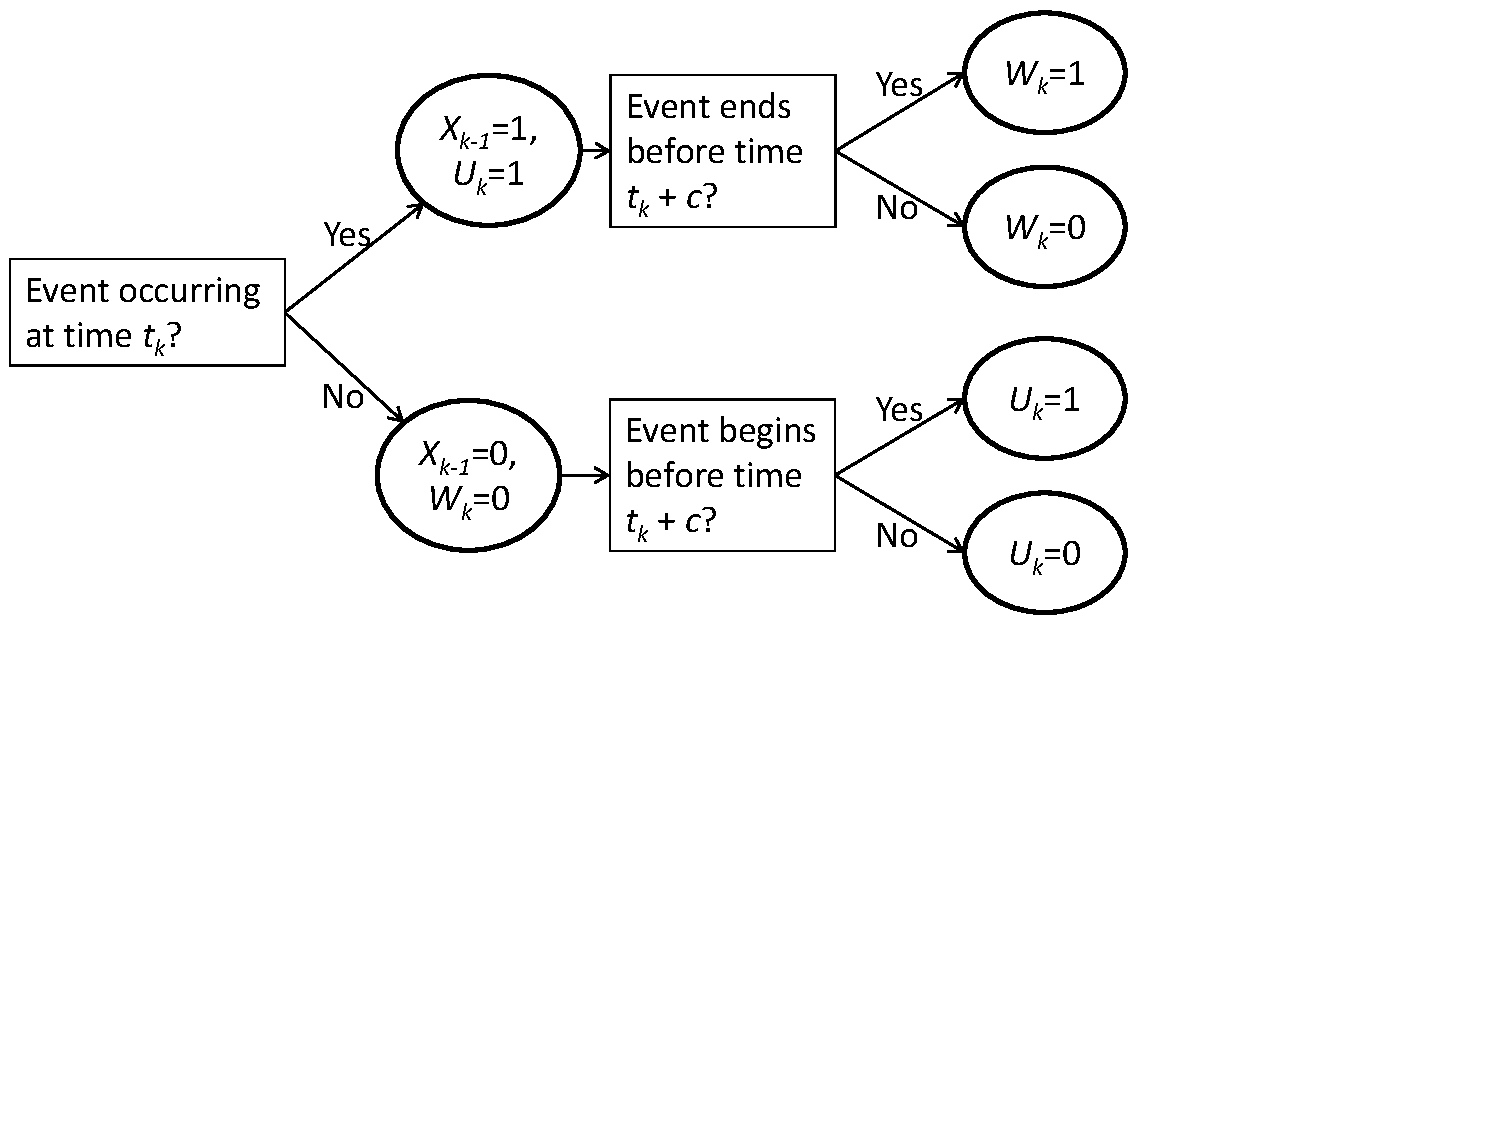
\includegraphics[clip=true, trim= 0 240 150 00, width=0.8\linewidth]{AIR_flowchart.pdf}
\caption{Procedure for combining MTS and interval recording}
\label{fig:questions}
\end{figure}  

The AIR procedure requires only marginally more effort on the part of the observer than an interval recording method used alone. 
One measure of effort is the level of sustained attention required on the part of the observer. Because the sustained attention needed for interval recording also entails the attention needed for momentary time sampling, the additional effort is minimal in this respect. 
Another measure of effort is the amount of data that must be recorded during the observation period. Because $W_k = 0$ is implied when $X_{k-1} = 0$ and $U_k = 1$ is implied when $X_{k-1} = 1$, AIR requires twice as much data as one of the single methods (rather than three times as much, might be supposed). 
Thus, for a fixed interval length, simultaneous use of all three methods entails at most twice as much effort as interval recording alone. 
Furthermore, using longer time-intervals with fewer intervals per observation period would mitigate the effort required.

Under the assumptions of the Alternating Poisson Process, the data generated by the AIR system can be modeled using a discrete-time Markov Chain, from which estimates of prevalence and incidence can be obtained. 
The Markov property of the Alternating Poisson Process implies that the joint distribution can be written as
\begin{multline}
\Pr\left(X_0=x_0,X_1=x_1,U_1 = u_1, W_1 = w_1,..., X_K=x_K, U_K = u_K, W_K = w_K \right) \\ = \Pr\left(X_0 = x_0\right) \prod_{k=1}^K \Pr\left(X_k = x_k, U_k = u_k, W_k = w_k | X_{k-1} = x_{k-1}\right). 
\end{multline}
Denote the transition probabilities $\Pr\left(X_k = b, U_k = c, W_k = d | X_{k-1} = a\right) = \pi_{a|bcd}$ and let $m_{a|bcd} = \sum_{k=1}^K I\left(X_{k-1} = a, X_k = b, U_k = c, W_k = d \right)$ for $a,b,c,d = 0,1$. 
Conditional on $X_0$, the log-likelihood of the observed AIR data is given by
\begin{equation}
\label{eq:AIR_loglik}
l_{AIR}\left(\phi,\zeta\right) = \sum_{a=0}^1 \sum_{b=0}^1 \sum_{c=0}^1 \sum_{d=0}^1 m_{a|bcd} \log \pi_{a|bcd}
\end{equation}
where
\begin{align*}
\pi_{0|000} &= \left[1 - p_0(d)\right]\exp\left(\frac{- \zeta c}{1 - \phi}\right) \\
\pi_{0|010} &= 1 - p_0(c + d) - \left[1 - p_0(d)\right]\exp\left(\frac{- \zeta c}{1 - \phi}\right) \\
\pi_{0|100} &= p_0(d)\exp\left(\frac{- \zeta c}{1 - \phi}\right) \\
\pi_{0|110} &= p_0(c + d) - p_0(d) \exp\left(\frac{- \zeta c}{1 - \phi}\right) \\
\pi_{1|010} &= 1 - p_1(c + d) - \left[1 - p_1(d)\right]\exp\left(\frac{- \zeta c}{\phi}\right) \\
\pi_{1|011} &= \left[1 - p_1(d)\right]\exp\left(\frac{- \zeta c}{\phi}\right) \\
\pi_{1|110} &= p_1(c + d) - p_1(d) \exp\left(\frac{- \zeta c}{\phi}\right) \\
\pi_{1|111} &= p_1(d)\exp\left(\frac{- \zeta c}{\phi}\right)
\end{align*}
and the remaining tansition probabilities are all equal to zero. 
See Appendix \ref{app:AIR_derivation} for the derivation of these quantities. 
As with PIR data, the MLEs $\hat\phi_{AIR}, \hat\zeta_{AIR}$ are obtained by maximizing $l_{AIR}$ using the Nelder-Mead algorithm. 

\section{Penalized likelihood estimators}

The previous section has illustrated that maximum likelihood estimates derived from MTS data or from interval recording data have undesirable operating characteristics when based on a moderate sample size of $K = 40$ intervals. 
In this section, we consider the use of penalized likelihood estimators (PLEs) to stabilize the behavior of the estimators and improve their performance in moderately sized samples. 
PLEs are derived by maximizing the sum of the log likelihood and a penalty term that depends on the parameters. 
Penalized likelihood estimation has been applied to an array of statistical problems where maximum likelihood methods break down, such as estimation of logistic regression coefficients in small samples \citep{Galindo-Garre2004bayesian, Gelman2008weakly}, estimation of correlation structure in high-dimensional multivariate regression models \citep{Warton2008penalized}, and estimation of variance components in multi-level models when the number of highest-level units is small \citep{Chung2012non-degenerate}. 

PLEs can be derived from a Bayesian perspective, by assigning a prior distribution to the model parameters and taking the posterior mode (given the prior and the data) as a point estimator \citep{Chung2012non-degenerate}. 
The penalty function is thus equivalent to the log of the prior distribution. 
An advantage of PLEs is that they provide a convenient and coherent way to incorporate into the estimation process prior information about the behavior. 

In most research contexts, we expect that prior knowledge about characteristics of the behavior will be more readily expressed in terms of the average event duration ($\mu$) and average interim time ($\lambda$). 
We therefore consider a class of priors in which $\mu$ and $\lambda$ follow independent gamma distributions, with \[
\mu \sim Gamma\left(\alpha_\mu, c \theta_\mu\right), \qquad \lambda \sim Gamma\left(\alpha_\lambda, c \theta_\lambda\right), \]
with hyperparameters $\alpha_\mu, \alpha_\lambda > 1$ and $\theta_\mu, \theta_\lambda > 0$. 
Note that the priors on $\mu$ and $\lambda$ are scaled in terms of the active interval length, so that they do not depend on the time unit in which the parameters and interval length are measured. 
This class of priors has the useful property that the implied priors on prevalence ($\phi$) and incidence ($\zeta$) have familiar distributional forms. 
Specifically, when $\theta_\mu = \theta_\lambda = \theta$, it follows that \[
\phi \sim Beta\left(\alpha_\mu, \alpha_\lambda \right), \qquad \zeta \sim Gamma^{-1}\left(\alpha_\mu + \alpha_\lambda, \frac{1}{c\theta} \right) \]
and that $\phi$ is independent of $\zeta$. 

The penalty function implied by these priors depends on how they are parameterized (i.e., based on priors for $\mu, \lambda$ or priors for $\phi, \zeta$). We recommend using the $\left(\mu,\lambda\right)$ parameterization because it reduces to zero when $\alpha_\mu = \alpha_\lambda = 1$ and $\theta_\mu = \theta_\lambda = \infty$, making the PLEs equivalent to the MLEs.
With this parameterization, the penalty function has the form 
\begin{equation}
p\left(\phi, \zeta\right) = \left(\alpha_\mu - 1\right) \log \left(\phi\right) + \left(\alpha_\lambda - 1\right) \log \left(1 - \phi\right) - \left(\alpha_\mu + \alpha_\lambda - 2\right) \log\left(\zeta\right) - \frac{\frac{\phi}{\theta_\mu} + \frac{1-\phi}{\theta_\lambda}}{c \zeta}.
\end{equation}
Given data based on recording system $s \in \{MTS, PIR, WIR, AIR\}$, the PLEs $\tilde\phi_s, \tilde\zeta_s$ are defined as the values that maximize $l_s\left(\phi, \zeta\right) + p\left(\phi, \zeta\right)$. 



Application of penalized likelihood estimators requires the analyst to choose values for the hyperparameters of the prior distribution. If one does not have specific prior knowledge regarding the characteristics of the behavior stream, it is prudent to choose hyperparameters that have little influence on the values of the PLEs. These weak priors imply a penalty function that is relatively flat, so that PLEs will correspond closely with the MLEs except when the data contain little information about the parameters. We suggest that $\alpha_\mu = \alpha_\lambda = 1.5$ and $\theta_\mu = \theta_\lambda = 10$ are reasonable default choices for hyperparameters. The priors are highest at $\mu = \lambda = 5 c$, or an average event duration and an average interim time of 5 intervals; the inter-quartile ranges are from $6.1 c$ to $20.5 c$. The implied prior for prevalence is symmetric about $\phi = 0.5$; its use amounts to adding the information from observing one independent moment where the probability of observing behavior is 0.5. We examine the empirical performance of the PLEs with these default hyperparameters in the next section.



In some research contexts, one may have fairly strong prior knowledge about certain behavioral characteristics, which can be used to inform the choice of hyperparameters. 
For example, prior experience with a class of behavior may suggest that it is unlikely for the average event duration to be more than two intervals in length, and that the most likely value for the average event duration is $\frac{1}{2}$ an interval length. 
This suggests choosing $\alpha_\mu = 3$ and $\theta_\mu = \frac{1}{4}$, so that the prior mode of $\mu$ is $\left(\alpha_\mu - 1\right) c \theta_\mu = \frac{c}{2}$ and $\Pr(\mu > 2c) < 0.02$.
Absent strong prior information about $\lambda$, one might use the default hyperparameters suggested above, taking $\alpha_\lambda = 1.5, \theta_\lambda = 10$. 

\section{Finite-sample performance}

We noted in a previous section that maximum likelihood estimates derived from MTS or PIR data are not always well-defined, even when the number of intervals is moderate. 
To remedy this problem, we have proposed the use of penalized likelihood estimates that are always well-defined and numerically stable. 
These approaches to estimation should produce equivalent results when based on very long observation sessions with many intervals of data, but they may differ when the number of intervals is more limited. 

Both maximum likelihood and penalized likelihood estimation represent alternatives to the standard method of summarizing intermittent behavioral observation data, which is to use the summary proportion of intervals with behavior. 
For MTS data, the summary proportion is an unbiased estimate of prevalence under a very broad class of data-generating models \citep{Rogosa1991statistical}; however, the summary proportion may be less efficient than the PLE or MLE for prevalence under the Alternating Poisson Process model. 
For PIR data, the summary proportion is biased as an estimate of prevalence \citep{Rogosa1991statistical}, while likelihood-based methods provide approximately unbiased estimates for sufficiently long observation sessions. 
Still, for a fixed sample size, the variability of the likelihood-based estimates may be worse than the bias in the summary proportion. It is therefore important to compare the accuracy of all of these estimators.

In order to understand the operating characteristics of the MLEs and PLEs in samples with a finite number of intervals, we conducted a computer simulation study. The simulations examined three specific questions: 
\begin{enumerate}
\item For a given recording procedure (MTS or PIR), how does the accuracy of the PLEs compare to the accuracy of the MLEs (for both prevalence and incidence) and the accuracy of the summary proportion (for prevalence only)? 
\item For a given recording procedure, how large a sample is needed to obtain approximately unbiased estimates of prevalence or incidence using penalized likelihood methods? 
\item How does the accuracy of estimates based on the novel AIR procedure compare to that of estimates based on MTS or PIR data? 
\end{enumerate}

\begin{table}[tb]
\centering
\caption{Simulation design}
\label{tb:simulation_design}
\begin{tabular}{clrrrr} \toprule
Parameter & Definition & Levels & Min. & Step & Max. \\ \midrule
$s$ & Recording system & 3 & \multicolumn{3}{c}{MTS, PIR, AIR} \\
$K$ & Session length & 15 & 10 & 10 & 150 \\
$\phi$ & Prevalence & 19 & 0.05 & 0.05 & 0.95 \\
$\zeta$ & Incidence & 10 & 0.05 & 0.05 & 0.50 \\
\bottomrule
\end{tabular}
\end{table}

Table \ref{tb:simulation_design} summarizes the simulation design.
We simulated data based on three different recording systems: MTS, PIR, and AIR; WIR was omitted because it is equivalent to using PIR for the absence of the behavior.
For MTS and PIR, we used $c = 1, d = 0$ and varied the length of the observation session from 10 to 150 intervals. 
This range spans a variety of situations in which intermittent behavioral observation recording might be used, from a quick observation in a classroom where the observer needs to capture the behaviors of several children to an intensive observation of a single child over the course of an entire class period. 
To provide for a fair comparison with the conventional recording systems, we simulated AIR data using $K / 2$ intervals of length $c = 2$ (i.e., twice as long as those for MTS or PIR). 
We varied the true prevalence of the behavior stream across nearly its entire possible range. 
Because $c = 1$ for MTS and PIR, incidence is scaled in terms of the length of an interval; for example, $\zeta = 0.1$ corresponds to an incidence of one new behavioral episode per ten intervals.
We varied incidence  between $\zeta = .05$ (one new behavior per 20 intervals) and $\zeta = .50$ (one new behavior every 2 intervals) because this represents a range of behaviors where intermittent recording procedures might feasibly be applied; in particular, PIR measurements would quickly approach ceiling levels when behaviors occur more frequently than once per two intervals. 

We implemented the simulations using the ARPobservation package \citep{Pustejovsky2014ARPobservation} for the R statistical computing environment \citep{RCoreTeam2014}. 
For each combination of parameter values ($\phi,\zeta,K$) and recording system, we generated 10000 behavior streams of length $K$ from an Alternating Poisson Process, then simulated data based on the specified recording system. 
For each string of simulated data, we calculated the summary proportion of intervals and then found the MLEs and PLEs using numerical maximization. 
For the PLEs, we used the default priors of $\alpha_\mu = \alpha_\lambda = 1.5$ and $\theta_\mu = \theta_\lambda = 10$.  

Depending on the research context, an analyst using these estimators might want to use the natural parameterization of $\phi$ and $\zeta$ or the transformed parameterization of $\logit(\phi)$ and $\log(\zeta)$, where $\logit(x) = \log(x) - \log (1 - x)$. 
The latter parameterization puts the scores on a scale from $-\infty$ to $\infty$, and so might be preferred by an analyst seeking to fit a linear model. 
Consequently, we studied each research question using both parameterizations. 
To address the first research question, we examined the root mean-squared error (RMSE) of the prevalence estimates and the relatively RMSE of the incidence estimates; we focused on relative RMSE, defined as $\E\left[\left(\hat\zeta - \zeta\right)^2\right] / \zeta$, because incidence is a rate. 
In the transformed parameterization, we examined the RMSE of $\logit(\phi)$ and $\log(\zeta)$.  

In addressing the second research question, regarding required minimum sample sizes to obtain approximately unbiased estimates, we used rather liberal criteria for bias. 
We believe that doing so is appropriate given the lack of alternative methods, particularly for estimating incidence. 
Our criteria for ``approximate unbiasedness'' are defined as follows. 
For prevalence, we used absolute bias in $\hat\phi$ of less than 0.03 and absolute bias in $\logit(\hat\phi)$ of less thann 0.05. 
For incidence, we used absolute relative bias in $\hat\zeta$ of less than 0.10 and absolute bias in $\log(\hat\zeta)$ of less than 0.10. \todo{Any further justifications for these bias criteria?} 



\subsection{Results: MTS}

\begin{knitrout}
\definecolor{shadecolor}{rgb}{0.969, 0.969, 0.969}\color{fgcolor}\begin{figure}[tb]


{\centering 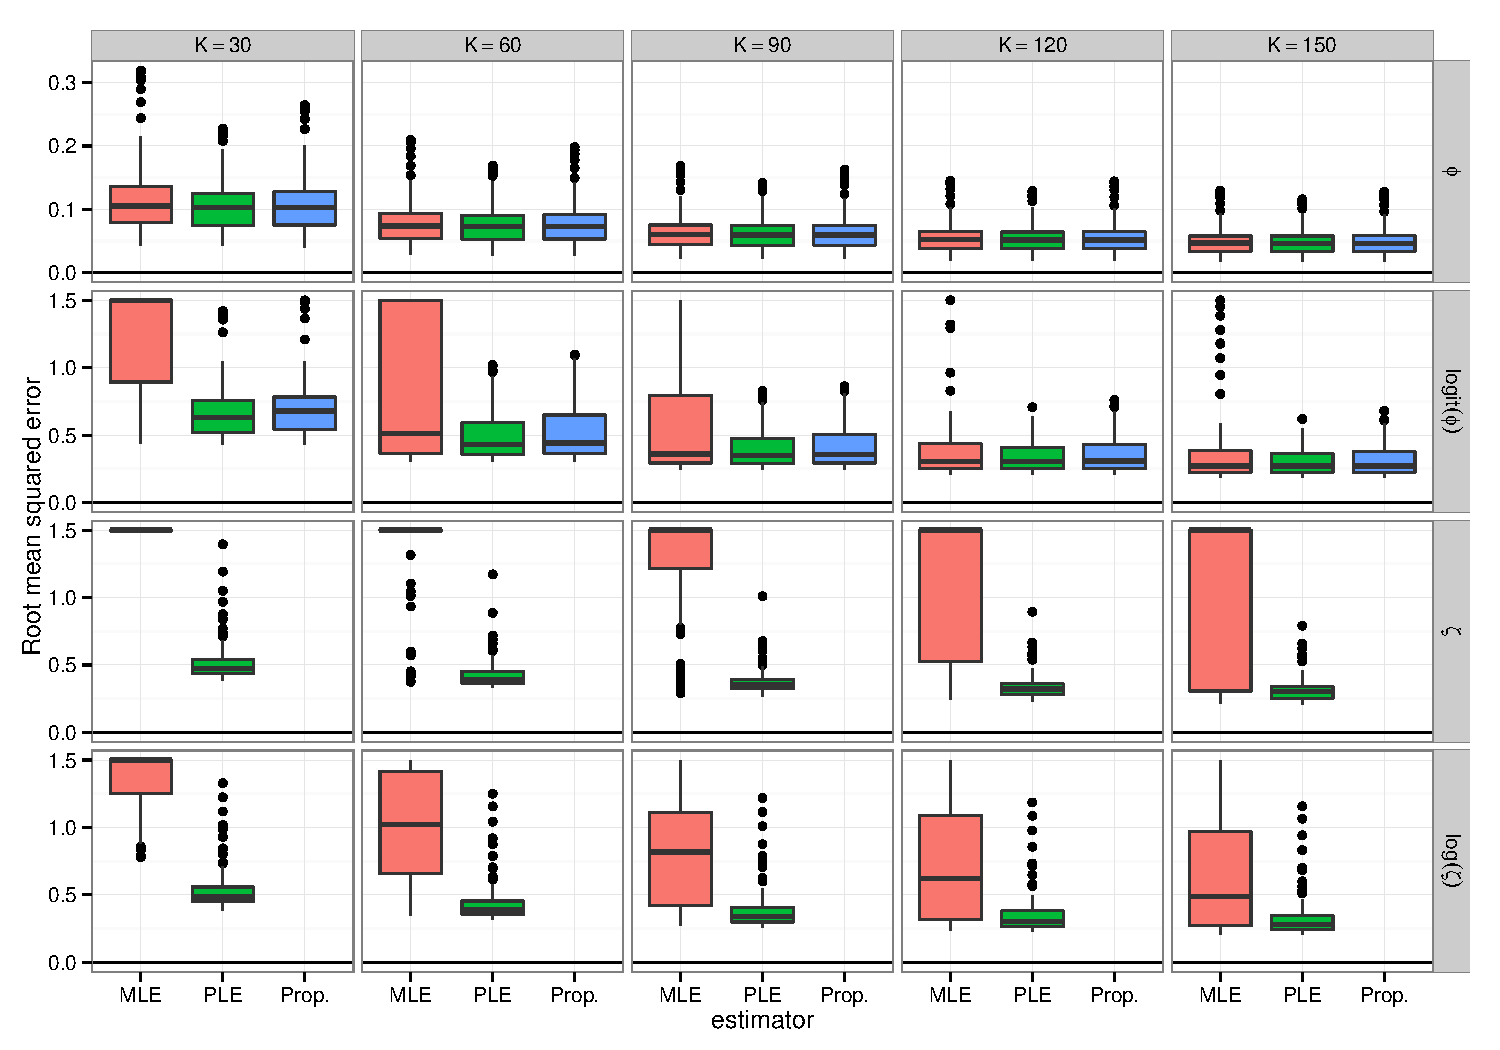
\includegraphics[width=\maxwidth]{fig/MTS_RMSE} 

}

\caption[Distribution of root mean-squared error of MLE, PLE, and summary proportion (Prop]{Distribution of root mean-squared error of MLE, PLE, and summary proportion (Prop.) estimates based on MTS data, across range of $0.05 \leq \phi \leq 0.95$ and $0.05 \leq \zeta \leq 0.50$. Values above 1.5 are not displayed. For $\zeta$, the root mean-squared error is relative to the true value.\label{fig:MTS_RMSE}}
\end{figure}


\end{knitrout}

Figure \ref{fig:MTS_RMSE} illustrates the distribution of RMSE of the MLEs, PLEs, and summary proportions based on MTS data, for varying levels of $K$; each row of graphs corresponds to a different parameter. 
Given that the MTS proportions are known to be unbiased estimates of prevalence, those estimates provide a point of reference for the accuracy of the MLEs and PLEs. 
Across all levels of $K$, the MLEs of $\phi$ have comparable RMSEs to the MTS proportions. 
However, the MLEs perform notably worse in terms of $logit(\phi)$ until $K = 120$ or more, a very large number of intervals.
Across the range of $K$, the PLEs of $\phi$ and $logit(\phi)$ have RMSE comparable to or smaller than the MTS proportions. 
In terms of both $\zeta$ and $log(\zeta)$, the MLEs perform considerably worse than the PLEs across all levels of $K$. 
However, the PLEs for $\zeta$ still have rather large relative RMSE (and similarly, the PLEs for $\log(\zeta)$ have large RMSE) for some parts of the parameter space.\todo{Characterize where in the parameter space PLEs don't perform well--is it small $\zeta$?}

\begin{knitrout}
\definecolor{shadecolor}{rgb}{0.969, 0.969, 0.969}\color{fgcolor}\begin{figure}[tb]


{\centering 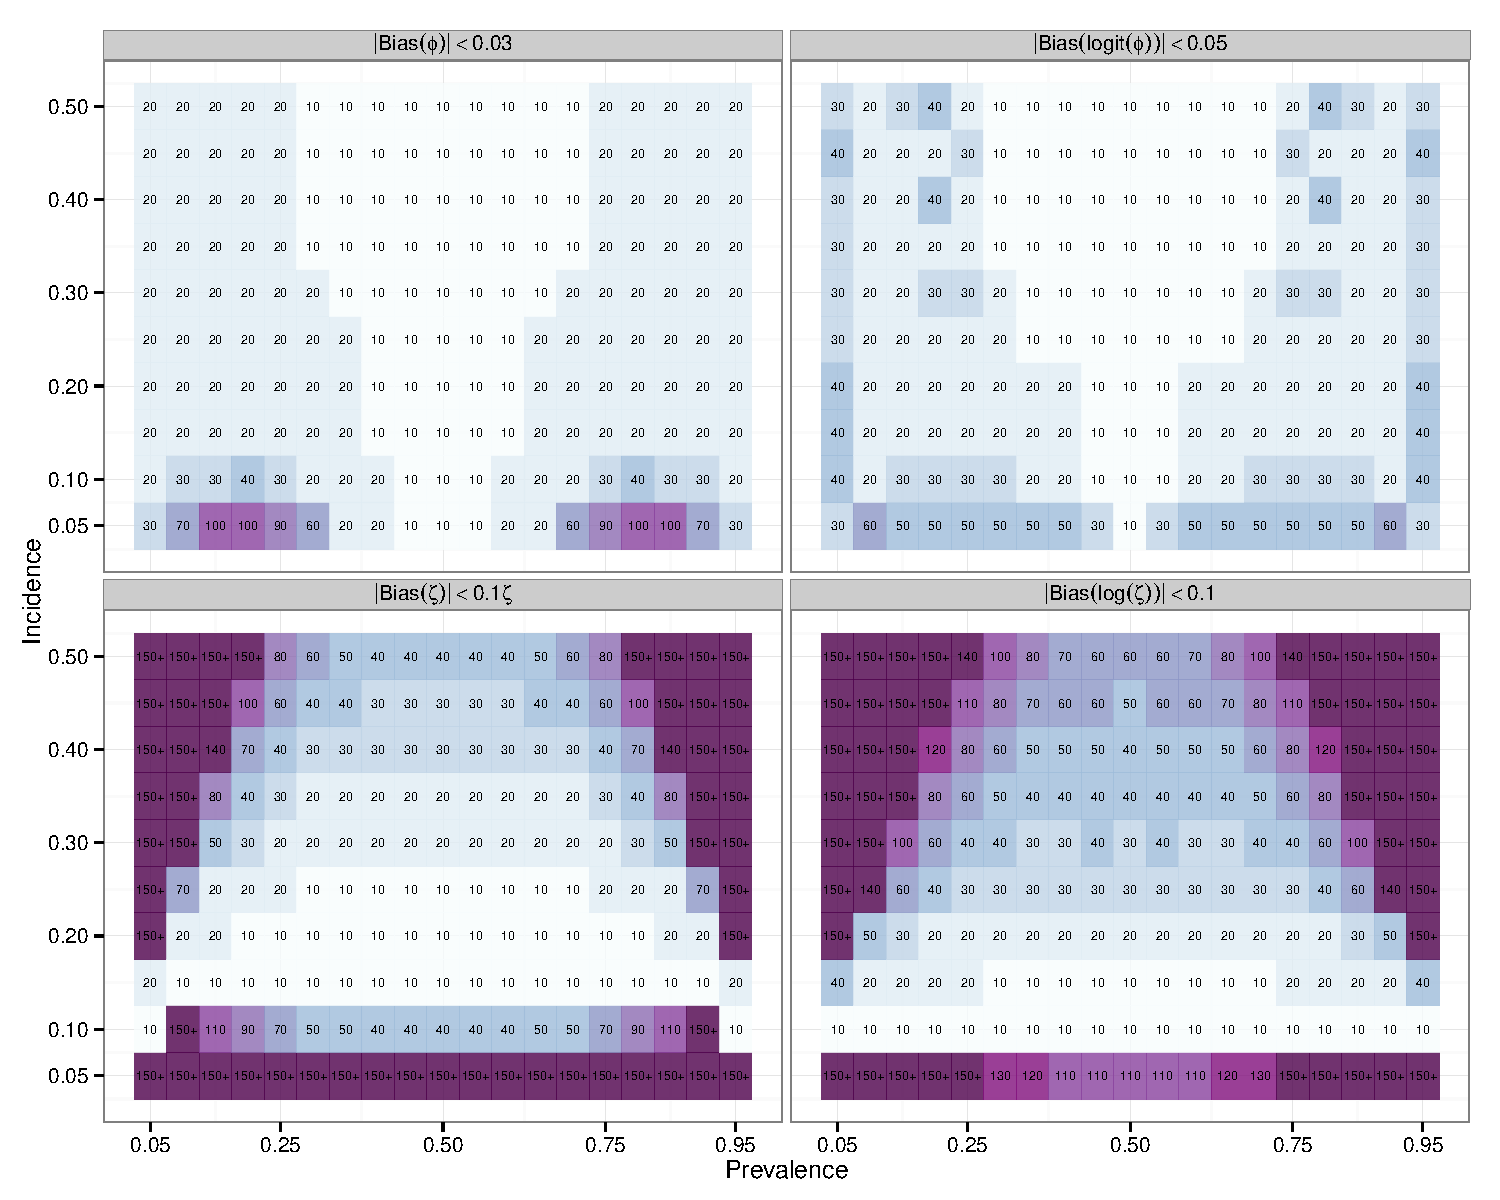
\includegraphics[width=\maxwidth]{fig/MTS_sample_size} 

}

\caption[Minimum number of MTS intervals required to obtain PLEs with absolute bias less than given criteria]{Minimum number of MTS intervals required to obtain PLEs with absolute bias less than given criteria.\label{fig:MTS_sample_size}}
\end{figure}


\end{knitrout}

Figure \ref{fig:MTS_sample_size} illustrates the minimum value of $K$ required to obtain PLEs with low bias. 
In terms of $\phi$ and $\logit(\phi)$, the estimator requires at most 40 intervals when the behavior is not too infrequent (i.e., $\zeta \geq 0.1 c$).
Even when $\zeta$ drops to $0.05 c$, low-bias estimates of $logit(\phi)$ can be obtained when $K \geq 60$. 
In terms of $\zeta$ and $\log(\zeta)$, low-bias estimates can be obtained when $K$ is at least 80 so long as the behavior has moderate prevalence ($0.30 \leq \phi \leq 0.70$) and incidence that is neither infrequent nor very frequent ($0.10 \leq \zeta \leq 0.45$). 
However, larger samples are required to obtain good incidence estimates when the behavior has more extreme prevalence and high incidence, or when the behavior has very low incidence.\todo{Add summary statement.}

\subsection{Results: PIR}

\begin{knitrout}
\definecolor{shadecolor}{rgb}{0.969, 0.969, 0.969}\color{fgcolor}\begin{figure}[tb]


{\centering 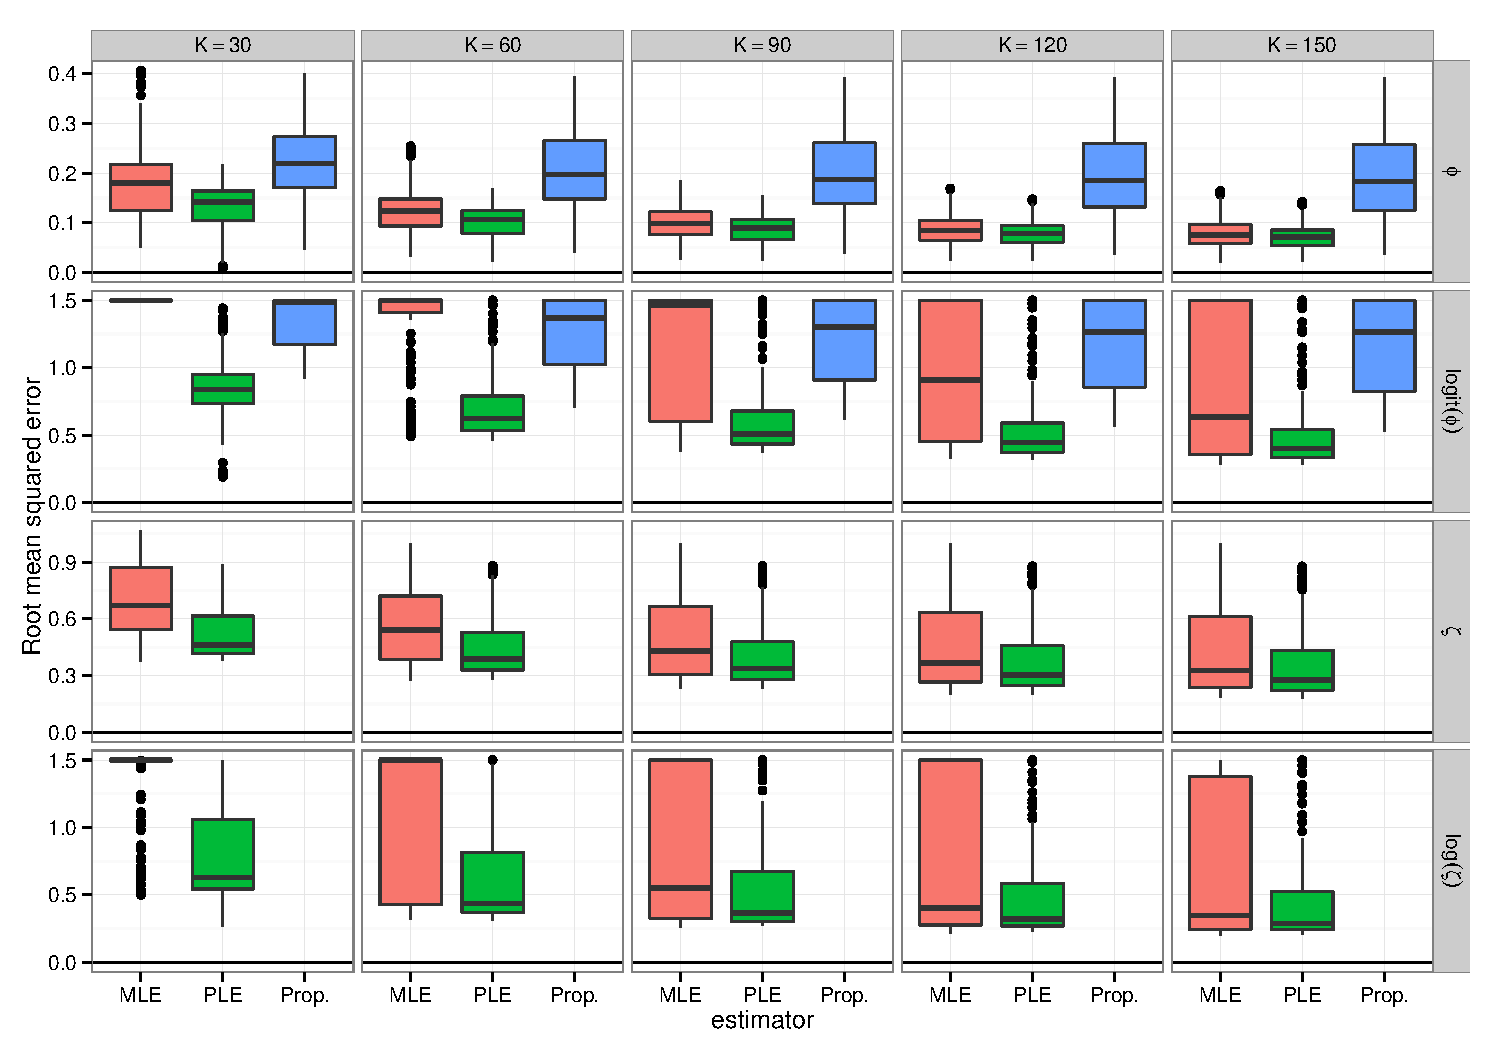
\includegraphics[width=\maxwidth]{fig/PIR_RMSE} 

}

\caption[Distribution of root mean-squared error of MLE, PLE, and summary proportion (Prop]{Distribution of root mean-squared error of MLE, PLE, and summary proportion (Prop.) estimates based on PIR data, across range of $0.05 \leq \phi \leq 0.95$ and $0.05 \leq \zeta \leq 0.50$. Values above 1.5 are not displayed. For zeta, the root mean-squared error is relative to the true value.\label{fig:PIR_RMSE}}
\end{figure}


\end{knitrout}

Figure \ref{fig:PIR_RMSE} illustrates the distribution of RMSE of the MLEs, PLEs, and summary proportions based on PIR data, across varying levels of $K$ and for each parameterization. 
In contrast to MTS, the PIR summary proportion performs quite poorly as an estimate of prevalence. 
For prevalence, the PLE performs notably better than both the MLE and the summary proportions across the entire range of $K$, in terms of both the natural parameterization and the transformed parameterization. 
For incidence, the PLEs once again provide more accurate estimates than the MLEs, in both parameterizations. 

Figure \ref{fig:PIR_sample_size} illustrates the minimum value of $K$ required for the PLEs based on PIR data to have low bias. 
The subset of the parameter space where one can obtain approximately unbiased estimates of prevalence with a moderate number of intervals is much smaller than with the MTS estimates. 
In terms of the bias of $\phi$, unbiased estimates can be obtained when $K$ is at least 70 and $0.10 \leq \phi \leq 0.35$ and $\zeta/c \leq 0.4$. 
Unbiased estimates can also be obtained when $K$ is at least 60 and $\phi \leq 0.80$ and $\zeta/c \leq 0.25$. In terms of $logit(\phi)$, unbiased estimates can be obtained when $K$ is at least 70 and $0.15 \leq \phi \leq 0.35$ and $\zeta/c \leq 0.30$. 
Unbiased estimates can also be obtained when $K$ is at least 90 and $\phi \leq 0.70$ and $\zeta/c \leq 0.15$. 
In order to obtain unbiased estimates of incidence, much larger values of $K$ are required. 
In terms of $\zeta$, unbiased estimates can be obtained when $K$ is at least 130 and $0.10 \leq \phi \leq 0.35$ and $\zeta \leq 0.45$. 
Unbiased estimates can also be obtained when $K$ is at least 130, and $\phi \leq 0.60$ and $\zeta/c \leq 0.25$. 
In terms of $log(\zeta)$, unbiased estimates can be obtained when $K$ is at least 140 and $\phi \leq 0.40$ and $\zeta \leq 0.35$.\todo{Re-write this paragraph in broader, less technical terms--e.g., "estimation of incidence from PIR data will generally require very large samples unless the behavior is known to have prevalence less than X and incidence less than X." See the comparable paragraph on MTS above.}

\begin{knitrout}
\definecolor{shadecolor}{rgb}{0.969, 0.969, 0.969}\color{fgcolor}\begin{figure}[tb]


{\centering 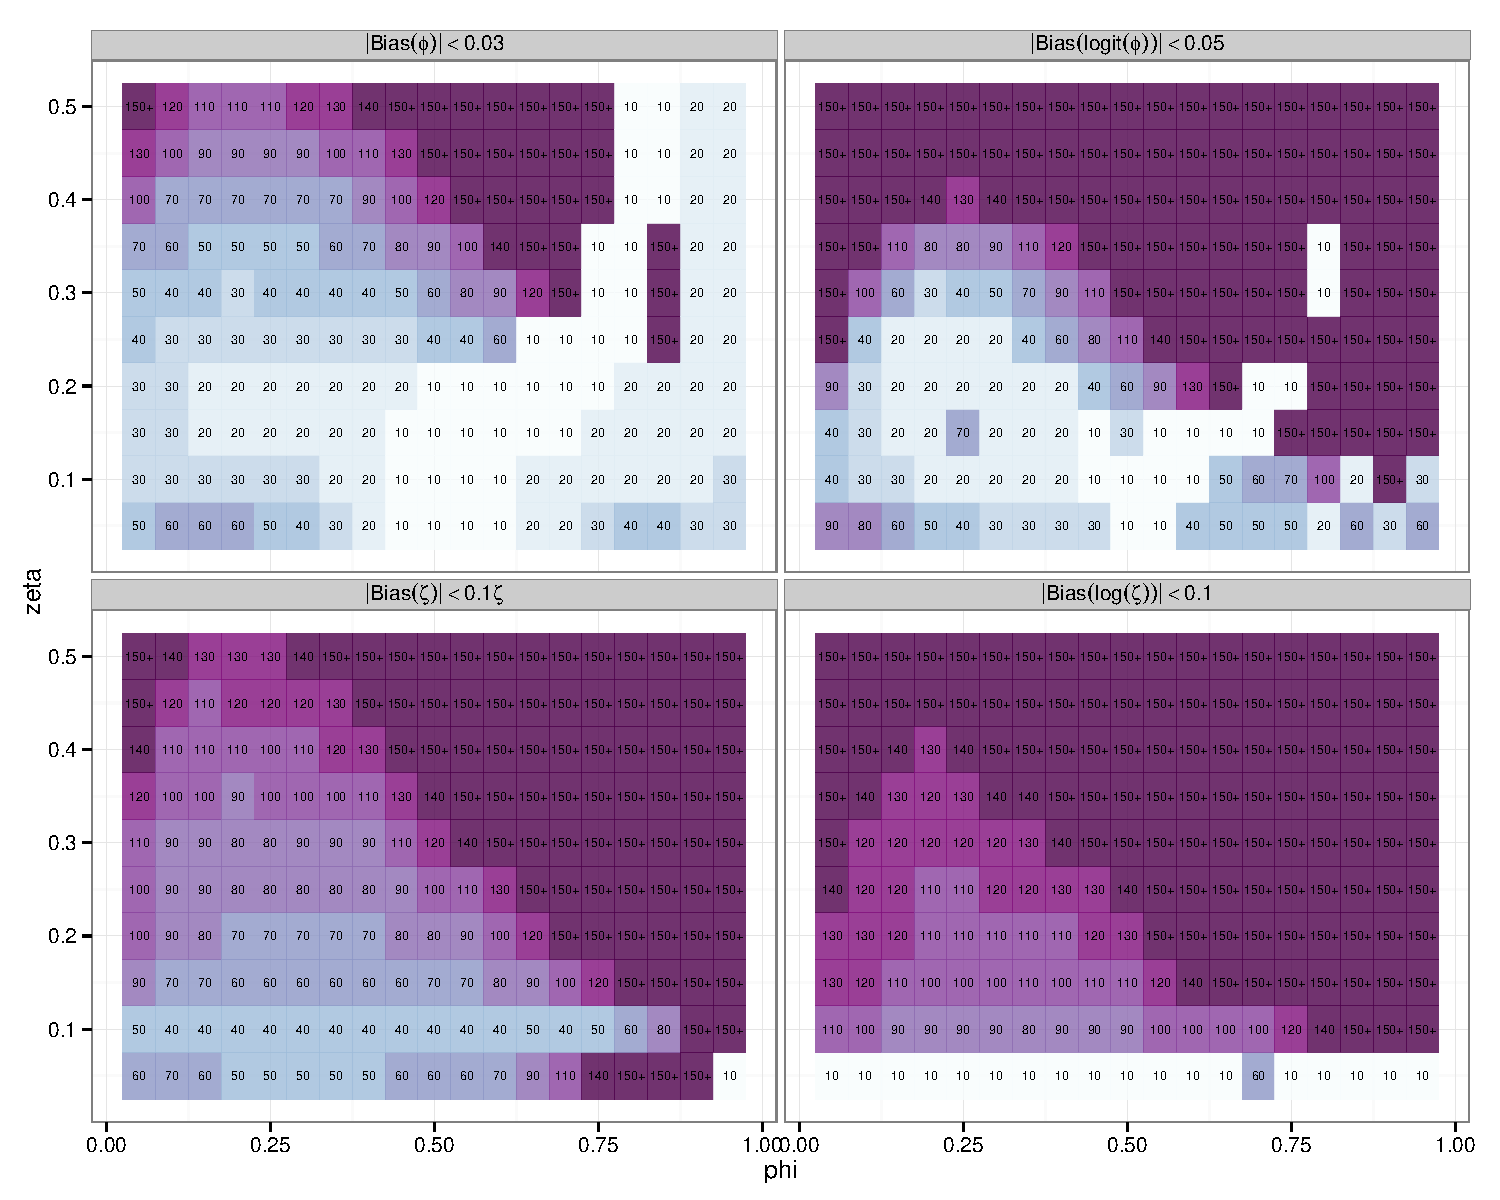
\includegraphics[width=\maxwidth]{fig/PIR_sample_size} 

}

\caption[Minimum number of PIR intervals required to obtain PLEs with absolute bias less than given criteria]{Minimum number of PIR intervals required to obtain PLEs with absolute bias less than given criteria.\label{fig:PIR_sample_size}}
\end{figure}


\end{knitrout}

\subsection{Results: AIR}

\begin{knitrout}
\definecolor{shadecolor}{rgb}{0.969, 0.969, 0.969}\color{fgcolor}\begin{figure}[tb]


{\centering 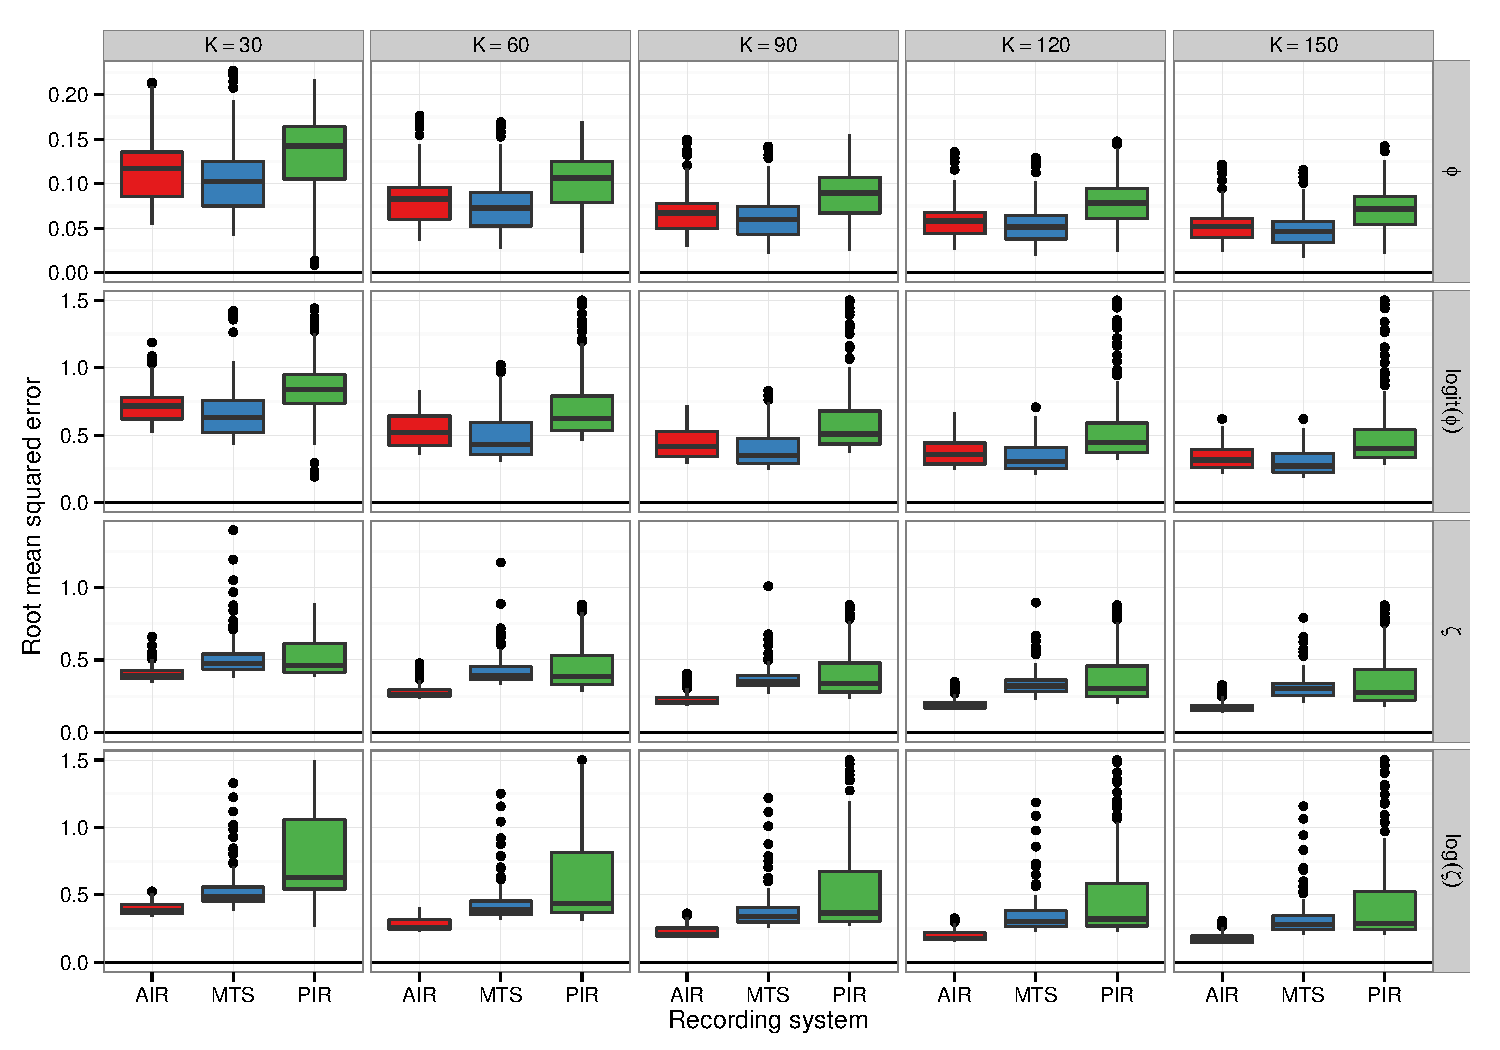
\includegraphics[width=\maxwidth]{fig/AIR_RMSE} 

}

\caption[Distribution of root mean-squared error of MLEs and PLEs based on AIR data, across range of $0]{Distribution of root mean-squared error of MLEs and PLEs based on AIR data, across range of $0.05 \leq \phi \leq 0.95$ and $0.05 \leq \zeta \leq 0.50$. Values above 1.5 are not displayed. For $\zeta$, the root mean-squared error is relative to the true value.\label{fig:AIR_RMSE}}
\end{figure}


\end{knitrout}

\begin{knitrout}
\definecolor{shadecolor}{rgb}{0.969, 0.969, 0.969}\color{fgcolor}\begin{figure}[]


{\centering 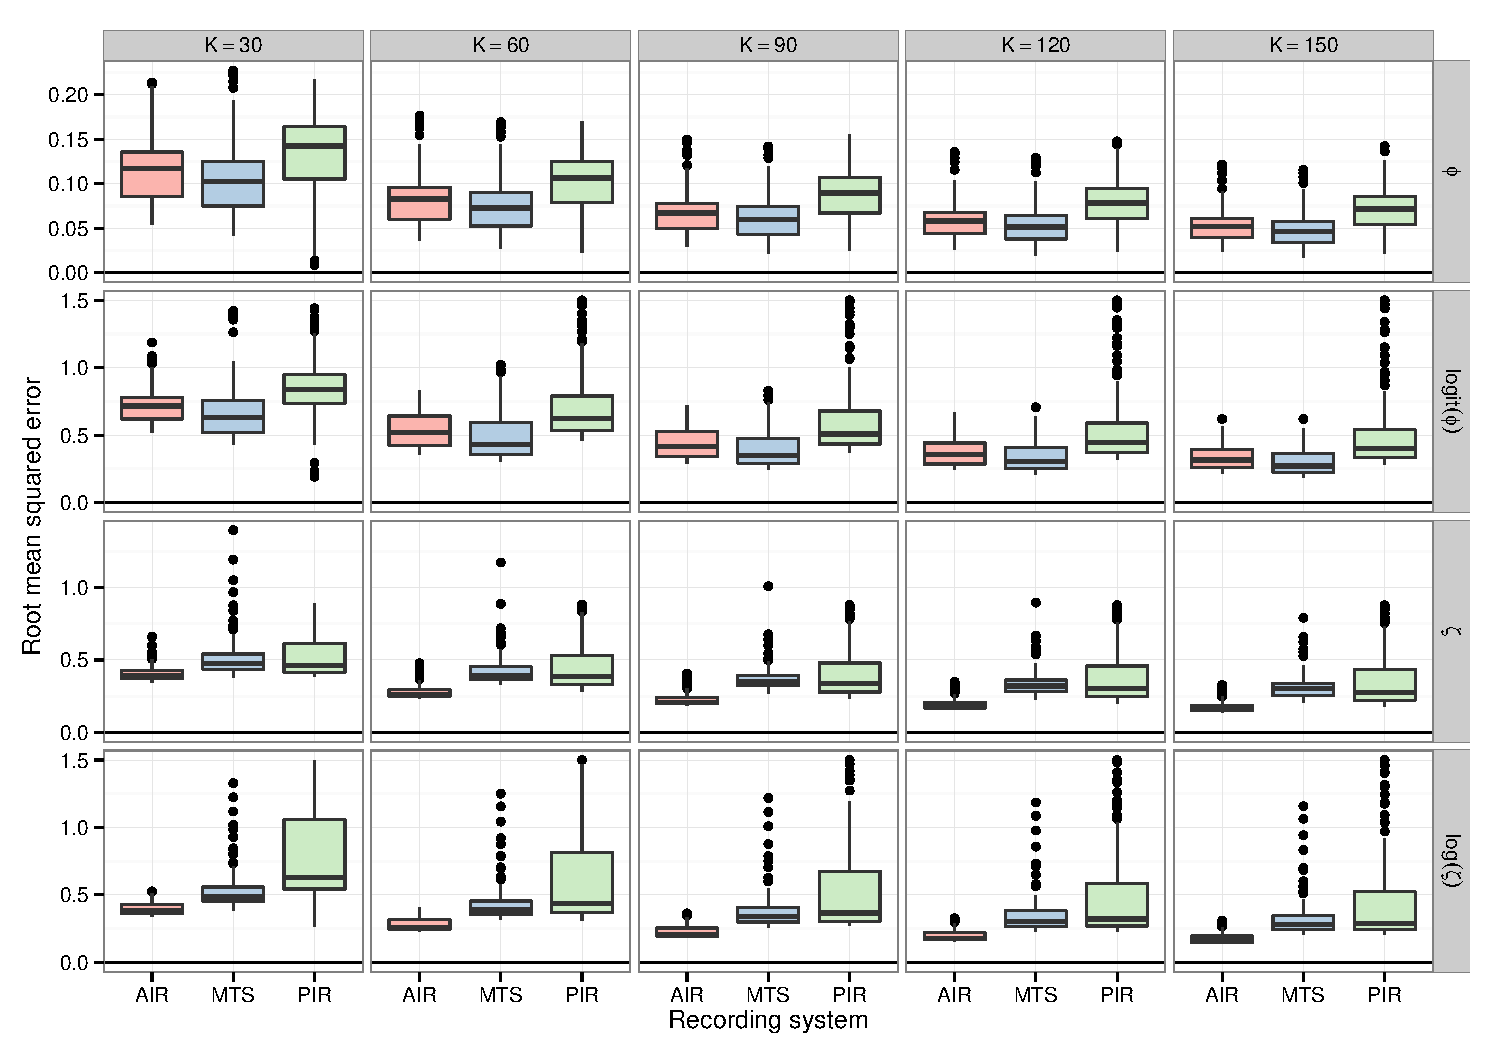
\includegraphics[width=\maxwidth]{fig/Method_RMSE} 

}

\caption[Distribution of root mean-squared error of PLE estimates based on AIR, MTS, and PIR data, across range of $0]{Distribution of root mean-squared error of PLE estimates based on AIR, MTS, and PIR data, across range of $0.05 \leq \phi \leq 0.95$ and $0.05 \leq \zeta \leq 0.50$. Values above 1.5 are not displayed. For zeta, the root mean-squared error for is relative to the true value.\label{fig:Method_RMSE}}
\end{figure}


\end{knitrout}

\begin{knitrout}
\definecolor{shadecolor}{rgb}{0.969, 0.969, 0.969}\color{fgcolor}\begin{figure}[tb]


{\centering 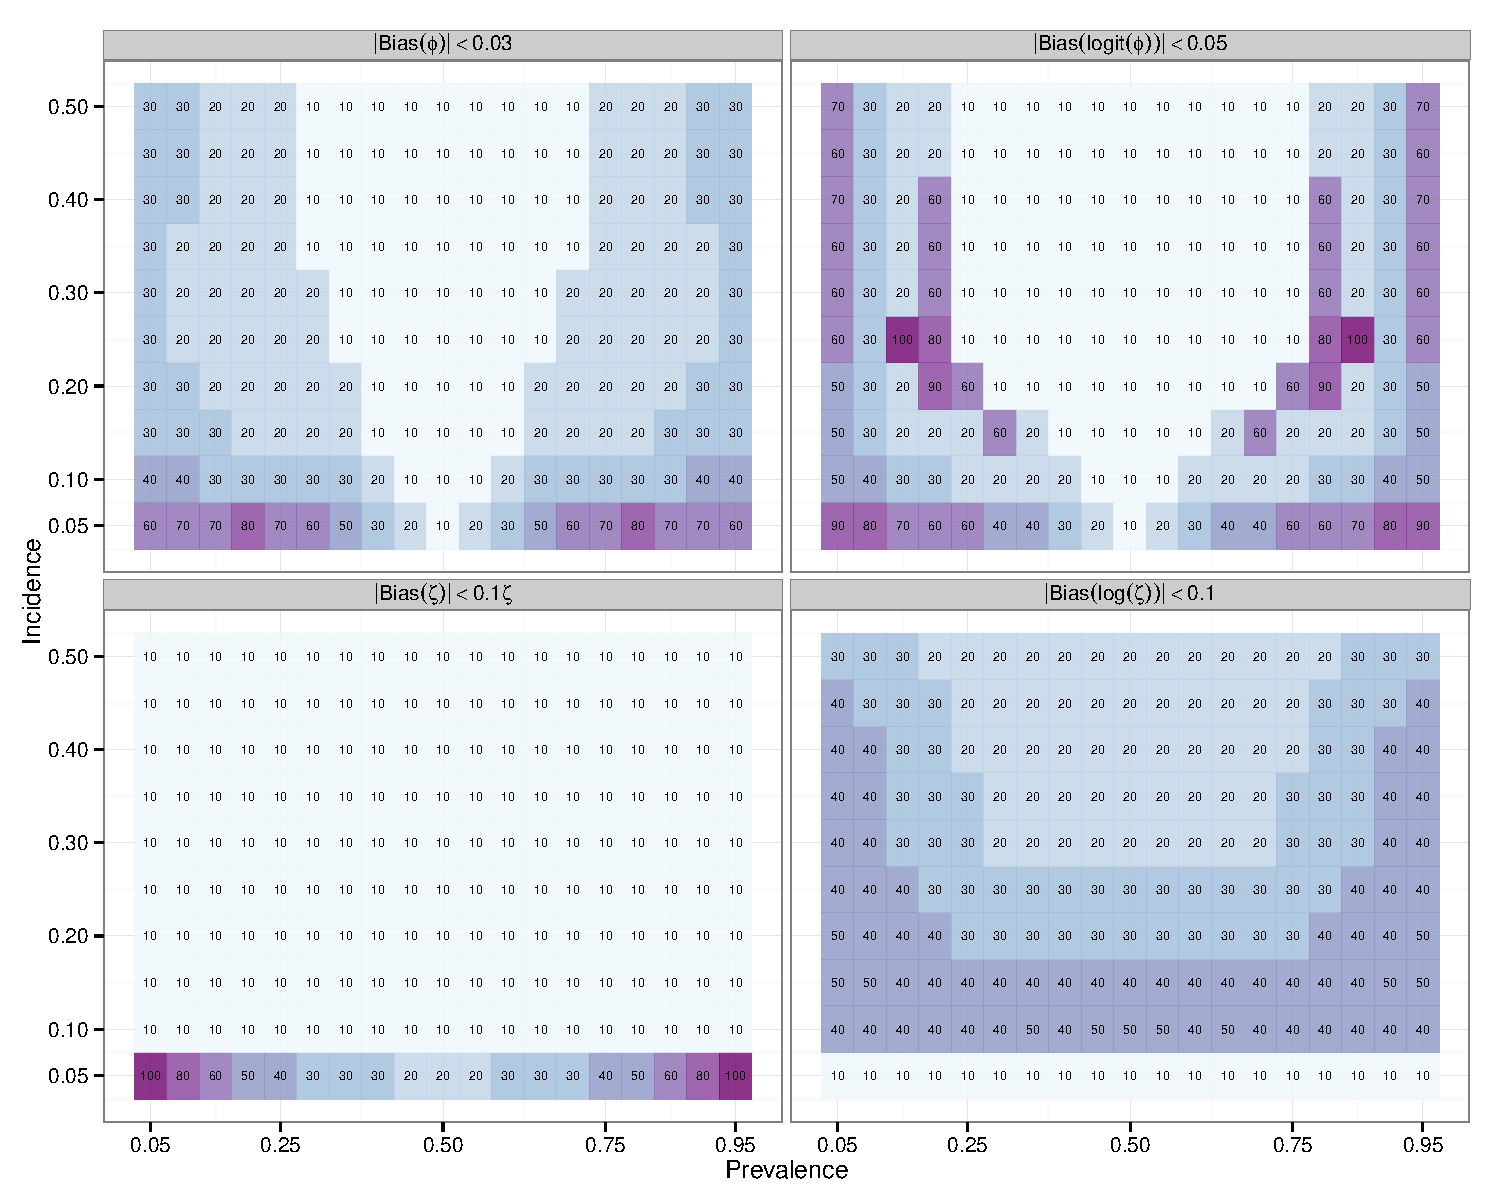
\includegraphics[width=\maxwidth]{fig/AIR_sample_size} 

}

\caption[Minimum observation session length required to obtain PLEs based on AIR data with absolute bias less than given criteria]{Minimum observation session length required to obtain PLEs based on AIR data with absolute bias less than given criteria.\label{fig:AIR_sample_size}}
\end{figure}


\end{knitrout}

\section{Application}
\label{sec:application}



This section demonstrates the use of the PLEs with empirical behavioral observation data. The data are drawn from \citet{Johnson2014reliability}. 
In this study, trained raters watched six scripted, pre-recorded, ten-minute videos of a classroom during a lesson. 
The script outlined when students in the classroom were to act academically engaged or to act disruptively. 
For each video, academic engagement behavior was coded using three different recording systems: MTS, PIR, and WIR. 
All three systems used 15 s intervals, yielding a total of 40 intervals per scored clip.
Each video clip was independently coded by ten different raters using each of the recording systems. 

The goal of our analysis is to estimate the prevalence and incidence of the behavior observed in each video clip, using the data from each of the three recording systems. 
Because each video was scored separately using each system, comparing the PLEs obtained from each type of data allows us to characterize the relative strengths and weaknesses of the observation recording methods. The fact that each clip is scored by multiple raters also allows us to observe a source of measurement error that the Alternating Poisson Process model does capture: ``inter-rater'' error, due the human observers not perfectly following the scoring procedure or not perceiving the behavior stream with perfect accuracy.

\begin{knitrout}
\definecolor{shadecolor}{rgb}{0.969, 0.969, 0.969}\color{fgcolor}\begin{figure}[tb]


{\centering 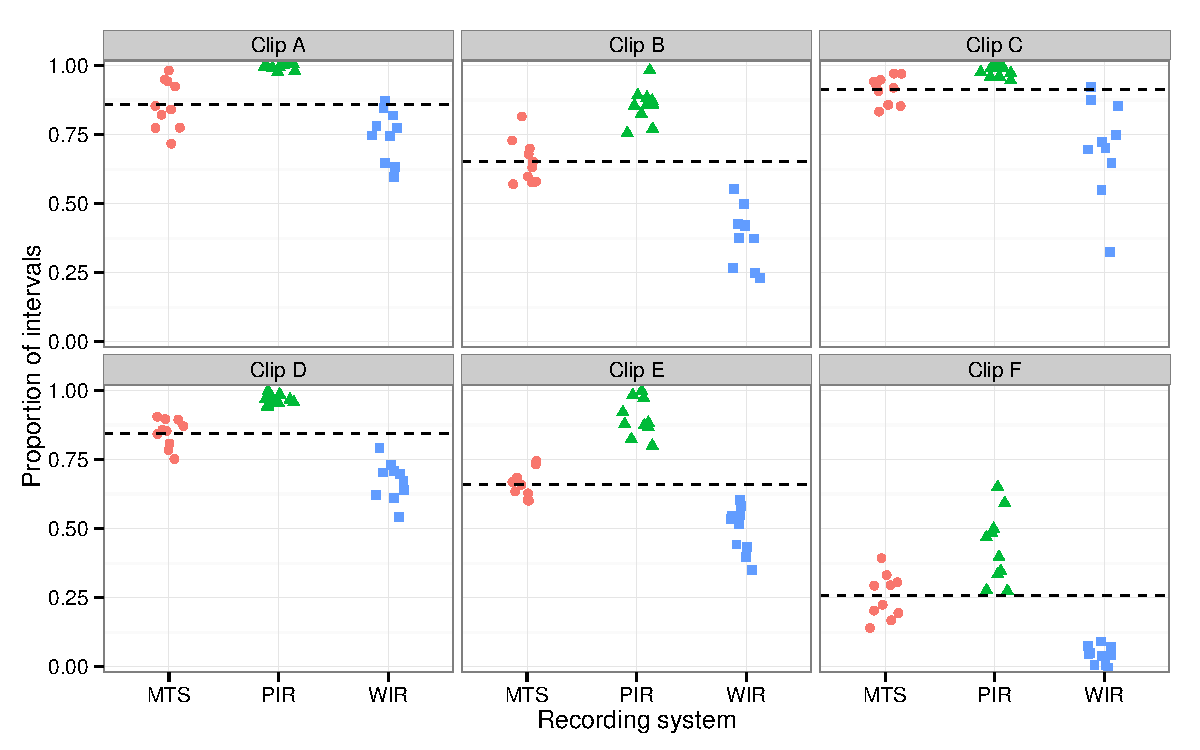
\includegraphics[width=\maxwidth]{fig/summary_prop} 

}

\caption[MTS, PIR, and WIR summary proportions for each rater, by clip]{MTS, PIR, and WIR summary proportions for each rater, by clip. Horizontal dashed lines correspond to the average MTS summary proportions.\label{fig:summary_prop}}
\end{figure}


\end{knitrout}

Figure \ref{fig:summary_prop} plots the overal proportion of intervals with academic engagment for each clip and each recording procedure, with separate points for each rater. The horizontal dashed lines represent the average of the MTS proportions across all ten raters, which we treat as a benchmark for the prevalence estimates based on the Alternating Poisson Process. The PIR proportions are almost all higher than the unbiased MTS proportions, while the WIR proportions are nearly always lower, which is consistent with the fact that the PIR summary proportion is an upwardly biased estimate of prevalence while the WIR proportion is a downwardly biased estimate of prevalence. The prevalence of academic engagement is quite high--above .80--in clips A, C, and D. In these three clips, the PIR proportions are frequently at or very near to the ceiling level. 



\begin{knitrout}
\definecolor{shadecolor}{rgb}{0.969, 0.969, 0.969}\color{fgcolor}\begin{figure}[tb]


{\centering 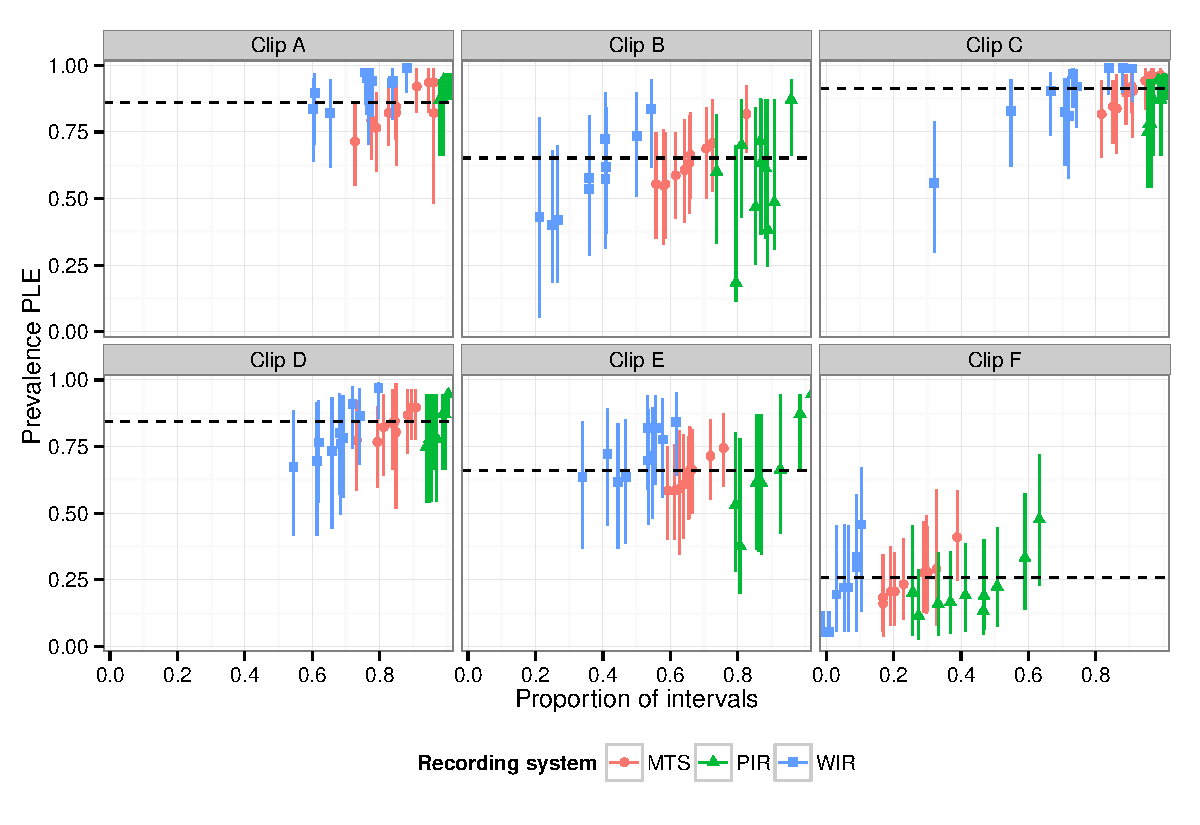
\includegraphics[width=\maxwidth]{fig/johnson_phi_est} 

}

\caption[PLE estimates of prevalence versus proportion of intervals with behavior, for each recording system and each rater]{PLE estimates of prevalence versus proportion of intervals with behavior, for each recording system and each rater. Vertical whisker bars correspond to 95\% confidence intervals for prevalence, obtained using a parametric bootstrapping procedure. Horizontal dashed lines correspond to the average MTS summary proportions.\label{fig:johnson_phi_est}}
\end{figure}


\end{knitrout}

Figure \ref{fig:johnson_phi_est} displays the PLEs for prevalence based on the MTS, PIR, and WIR scores for each rater and each clip. 
The prevalence estimates are plotted on the vertical axis, with the corresponding summary proportion of intervals on the horizontal axis. 
The quality of the estimates varies substantially by both recording procedure and by clip. 
For MTS, the PLEs are all close to the raw proportions (which are unbiased estimates of prevalence). 
The MTS confidence intervals cover the benchmark prevalence estimate in 58 out of the 60 MTS records and are generally narrower than the confidence intervals based on the PIR and WIR data.
The PLEs based on PIR and WIR are in roughly in the same range as the estimates based on MTS data. 
Thus, on a gross level, the PLEs appear to correct the over- or under-estimation of prevalence in the summary proportions. 
The confidence intervals based on PIR data cover the benchmark prevalence estimate in 48 out of the 60 total records, with most of the discrepancies occurring in clip A, where many of the the PIR records are at ceiling. 
Similarly, the confidence intervals based on WIR data cover the benchmark prevalence estimate in 52 out of 60 records. 
However, the PIR and WIR estimates are generally considerably less precise than the MTS estimates, with much wider confidence intervals.\todo{Provide numerical comparison of CI width.}

\begin{knitrout}
\definecolor{shadecolor}{rgb}{0.969, 0.969, 0.969}\color{fgcolor}\begin{figure}[tb]


{\centering 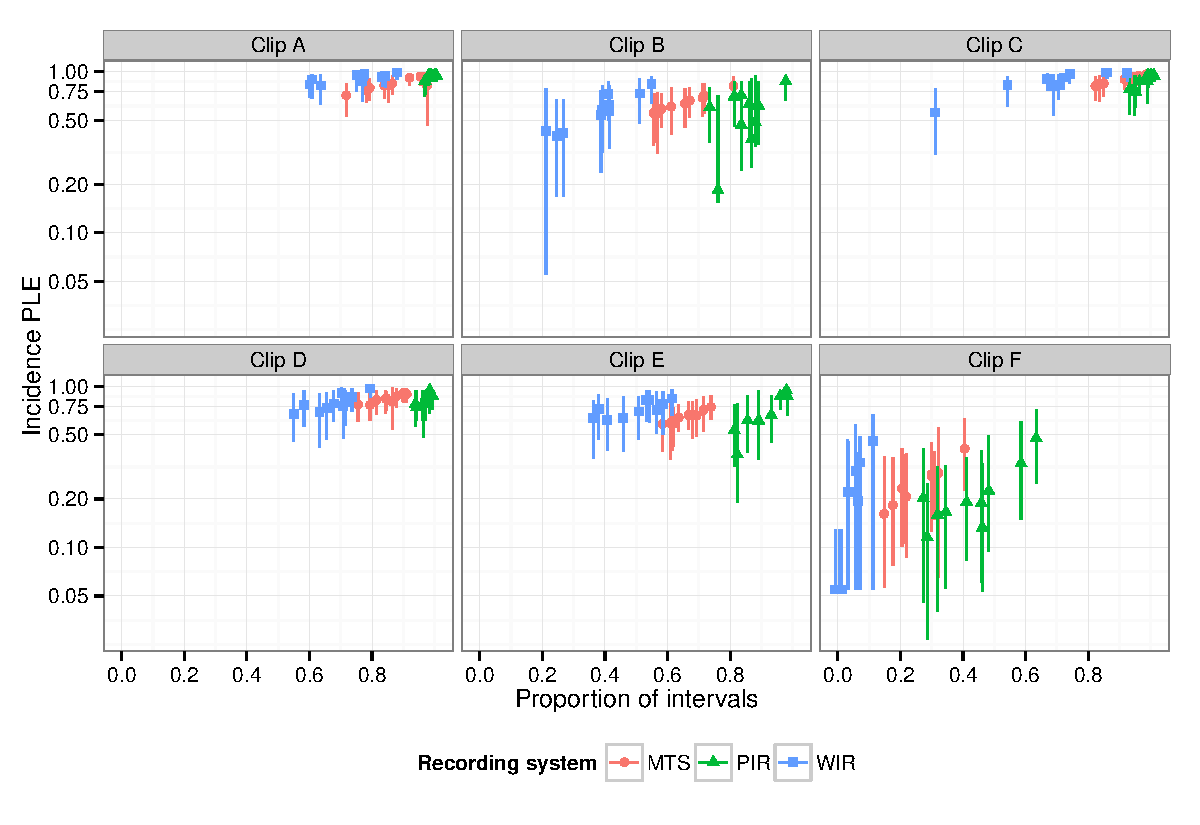
\includegraphics[width=\maxwidth]{fig/johnson_zeta_est} 

}

\caption[PLE estimates of incidence versus proportion of intervals with behavior, for each recording system and each rater]{PLE estimates of incidence versus proportion of intervals with behavior, for each recording system and each rater. Vertical whisker bars correspond to 95\% confidence intervals for incidence, obtained using a parametric bootstrapping procedure.\label{fig:johnson_zeta_est}}
\end{figure}


\end{knitrout}

Figure \ref{fig:johnson_zeta_est} displays the penalized likelihood estimates of incidence for each rater and each clip, again plotted against the raw proportion of intervals. Note that the vertical axis of this plot is on the log scale. 
In clips A through E, the estimates of the incidence of academic engagement are very high, suggesting that the student cycled rapidly between episodes of engagement and disruption.\todo{Comment on Clip F.} 
However, based on the simulation evidence presented in the previous section, we do not have great confidence in these estimates. 
For the moderate sample size of $K = 40$, none of the recording methods provide reasonable estimates of incidence for behaviors with high prevalence ($\phi > 0.5$) and high incidence ($\zeta > 0.5$).
Unfortunately, we do not have any benchmark estimate of the true incidence of academic engagement in each of the clips. 
Lacking a credible point of comparison, we cannot directly evaluate the accuracy of the incidence estimates. 
We note only that the estimates from all three systems appear to be in rough agreement.
\todo[inline]{General discussion points?}

\section{Discussion}
\label{sec:discussion}

In this paper, we have considered how to estimate the prevalence and incidence of a state behavior from data collected using conventional intermittent observation recording systems, including momentary time sampling, partial interval recording, and whole interval recording. Following earlier work by \citet{Brown1977estimation} on MTS, we used an Alternating Poisson Process to model the behavior stream as perceived by the observer, from which models for PIR, WIR, and AIR could be derived. For estimating the model parameters, simulation evidence indicated that penalized likelihood methods with generic, weak priors generally outperformed maximum likelihood methods--often dramatically so. For PIR data, penalized likelihood estimates of prevalence provided much more accurate estimates than the naiv\"e summary proportion, which is currently widely used.

We have also described a novel recording procedure, augmented interval recording, that involves combining MTS, PIR, and WIR. For a given period of observation, and using intervals twice the length of other procedures, AIR provides estimates of prevalence that are only slightly less accurate than estimates based on MTS, while also providing estimates of incidence that are substantially more accurate than estimates based on any other procedure. Of course, at present these advantages are only theoretical. To determine whether AIR offers any advantage in practice, its feasibility in real-life research contexts will need to be assessed.  

Across all of the recording procedures that we have considered, the foremost limitation of the models and estimation techniques that we have studied is the strength of the assumptions entailed by the Alternating Poisson Process model for the behavior stream. The model posits that the individual episodes of behavior and spans of time in between episodes are exponentially distributed. Whether these distributional assumptions are reasonable--and for what classes of behavior--is an important question requiring further empirical research. Addressing it will likely require measuring the behavior of a large sample of participants using intensive, continuous recording techniques. 
Another related avenue of further research is to examine the extent to which the proposed estimation techniques are robust to violations of the distributional assumptions (e.g., assuming that event durations follow a gamma distribution that has lower variance than the exponential). It may well be that the robustness of the PLEs depends on which system is used to record the data, and whether prevalence or incidence is of primary interest.

Several other limitations of these models should also be acknowledged. Our approach has treated the recording procedures themselves as essentially mechanical procedures that can be applied without human error, yet in practice the procedures are not perfectly reliable. Indeed, the data from \citet{Johnson2014reliability} displayed a surprisingly high level of inter-rater variability. The model we have considered could be seen as implicitly accomodating rater error by allowing that the Alternating Poisson Process describes the observer's \textit{perception} of the behavior stream, rather than the true behavior stream. How to extend the model in order to more explicitly account for human error in the recording process remains an open question for further research.

Another limitation of the models is that they are limited to describing measurement error from a single observation session. In practice, systematic behavioral observation data is often collected on a single participant across many sessions (as in a single-case study) or across many participants (as in a between-subjects experiment). In either setting, it would be useful to embed the measurement model that we have proposed in a generalized linear modeling framework, which could be used to describe changes in prevalence and incidence across time, or in a random-effects framework, which could be used to describe between-subjects variation in the characteristics of behavior streams.

Despite these limitations, the models and estimation methods that we have proposed remain useful. For MTS data, penalized likelihood provides a means to estimate incidence as well as to assess the extent of measurement error in the estimate of prevalence. For PIR data, the penalized likelihood estimates of prevalence represent an improvement over the current standard approach, which is to simply ignore the bias in the summary proportion. 

Though not the focus of the present paper, the models that we have described can also be applied to develop better psychometric guidance for behavioral observation data.\todo{Discuss Lane & Ledford (2014) and related work.} Through further mathematical analysis or though computer simulation, the models that we have presented could be used to study how choices regarding recording procedures, interval lengths, rest times, and observation session lengths influence the precision of behavioral measurements. Guidance regarding these aspects of study design would be useful to applied researchers designing single-case experiments or between-subjects trials.

\bibliographystyle{apacite}
\bibliography{\bibfile}
 
\appendix

\section{Derivation of PIR model}
\label{app:PIR_derivation}

The joint distribution of PIR observations depends on the conditional probabilities $\psi_k = \Pr\left[ Z(t_k) = 1 \left| U_1,...,U_{k-1}\right.\right]$. 
This appendix provides a derivation of Expression (\ref{eq:psi_k}) in terms of the parameters of the Alternating Poisson Process. The derivation will make use of the following lemma.

\begin{lemma}
\label{lemma1}
The conditional probabilities of $Z(t_k) = 1, U_{k-1} = 1$ given $Z(t_{k-1})$ are:
\begin{align*}
\Pr\left(Z(t_k) = 1, U_{k-1} = 1 \left| Z(t_{k-1}) = 1 \right.\right) &= p_1(c + d) \\
\Pr\left(Z(t_k) = 1, U_{k-1} = 1 \left| Z(t_{k-1}) = 0 \right.\right) &= p_0(c + d) - p_0(d) \exp\left(\frac{- \zeta c}{1 - \phi}\right).
\end{align*}
\end{lemma}

\begin{proof}
Observe that \[
\Pr\left(Z(t_k) = 1, U_{k-1} = 1 \left| Z(t_{k-1}) = 1 \right.\right) = \Pr\left(Z(t_k) = 1 \left| Z(t_{k-1}) = 1 \right.\right) = p_1(c + d) \]
and \begin{align*}
\Pr &\left(Z(t_k) = 1, U_{k-1} = 1 \left| Z(t_{k-1}) = 0 \right.\right) \\
& \qquad \qquad = \int_0^c\frac{p_1(c - t) \zeta}{(1 - \phi)}\exp\left(\frac{-\zeta t}{1 - \phi}\right) dt \\
& \qquad \qquad  = \phi \left[ 1 - \exp\left(\frac{- \zeta (c + d)}{\phi(1 - \phi)}\right) - \exp\left(\frac{- \zeta c}{1 - \phi}\right) + \exp\left(\frac{- \zeta (\phi c + d)}{\phi(1 - \phi)}\right)\right] \\
& \qquad \qquad = p_0(c + d) - p_0(d) \exp\left(\frac{- \zeta c}{1 - \phi}\right).
\end{align*}
\end{proof}

Turning to the derivation of $\psi_k$, begin by noting that $U_{k-1} = 0$ implies that $Z(t_k + c) = 0$. 
It follows from the Markov property that 
\begin{multline*}
\Pr\left(Z(t_k) = 1 \left| U_1 = u_1,...,U_{k-2} = u_{k-2}, U_{k-1} = 0 \right.\right) \\ 
= \Pr\left(Z(t_k) = 1 \left| Z(t_{k-1} + c) = 0 \right.\right) = p_0(d).
\end{multline*}
Next, Lemma \ref{lemma1} implies that \begin{multline*}
\Pr\left(Z(t_k) = 1, U_{k-1} = 1 \left| U_1,...,U_{k-2} \right.\right) \\
= \psi_{k-1} p_1(c + d) + (1 - \psi_{k-1}) \left[p_0(c + d) - p_0(d) \exp\left(\frac{- \zeta c}{1 - \phi}\right)\right].
\end{multline*}
It therefore follows that 
\begin{multline*}
\Pr\left(Z(t_k) = 1 \left| U_1 = u_1,...,U_{k-2} = u_{k-2}, U_{k-1} = 1 \right.\right) \\
= \frac{\psi_{k-1} p_1(c + d) + (1 - \psi_{k-1}) \left[p_0(c + d) - p_0(d) \exp\left(\frac{- \zeta c}{1 - \phi}\right)\right]}{1 - (1 - \psi_{k-1})\exp\left( \frac{-\zeta c}{1 - \phi}\right)}.
\end{multline*}
Thus, $\psi_k$ can be written as a function of $\psi_{k-1}$ and $u_{k-1}$, as given in (\ref{eq:psi_k}).

\section{Derivation of AIR model}
\label{app:AIR_derivation}

This appendix provides a derivation of the transition probabilities for the AIR model in terms of the parameters of the Alternating Poisson Process. Begin by noting that, by the definitions of the recording procedures, $X_{k-1} = 0$ implies that $W_k = 0$ and $X_{k-1} = 1$ implies that $U_k = 1$. It follows that $\pi_{0|bc1} = 0$ for $b,c = 0,1$ and $\pi_{1|b0d} = 0$ for $b,d=0,1$. Derivation of the other transition probabilities will make use of the following lemma. (The proof follow the same logic as in Lemma \ref{lemma1}, and is therefore omitted.)

\begin{lemma}
\label{lemma2}
The conditional probability of $Z(t_k) = 1, W_{k-1} = 0$ given that $Z(t_{k-1}) = 1$ is
\[
\Pr\left(Z(t_k) = 1, W_{k-1} = 0 \left| Z(t_{k-1}) = 1 \right.\right) = p_1(c + d) - p_1(d) \exp\left(\frac{- \zeta c}{\phi}\right). \]
\end{lemma}

Turning to the eight remaining transition probabilities, note that
\begin{align*}
\pi_{0|100} &= \Pr\left(X_k = 1, U_k = 0 | X_{k-1} = 0\right) \\
&= \Pr\left(X_k = 1 | Z(t_k + c) = 0\right) \Pr\left(U_k = 0 | X_{k-1} = 0\right) \\
&= p_0(d)\exp\left(\frac{- \zeta c}{1 - \phi}\right).
\end{align*}
Similarly,
\begin{align*}
\pi_{0|000} &= \Pr\left(X_k = 0, U_k = 0 | X_{k-1} = 0\right) = \left[1 - p_0(d)\right]\exp\left(\frac{- \zeta c}{1 - \phi}\right) \\
\pi_{1|111} &= \Pr\left(X_k = 1, W_k = 1 | X_{k-1} = 1\right) = p_1(d)\exp\left(\frac{- \zeta c}{\phi}\right) \\
\pi_{1|011} &= \Pr\left(X_k = 0, W_k = 1 | X_{k-1} = 1\right) = \left[1 - p_1(d)\right]\exp\left(\frac{- \zeta c}{\phi}\right).
\end{align*}
Next, it follows from Lemmas \ref{lemma1} and \ref{lemma2} that
\begin{align*}
\pi_{0|110} &= \Pr\left(X_k = 1, U_k = 1 | X_{k-1} = 0\right) = p_0(c + d) - p_0(d) \exp\left(\frac{- \zeta c}{1 - \phi}\right) \\
\pi_{1|110} &= \Pr\left(X_k = 1, W_k = 0 | X_{k-1} = 1\right) = p_1(c + d) - p_1(d) \exp\left(\frac{- \zeta c}{\phi}\right).
\end{align*}
The two remaining transition probabilities can be obtained by subtraction:
\begin{align*}
\pi_{0|010} &= 1 - \pi_{0|000} - \pi_{0|100} - \pi_{0|110} = 1 - p_0(c + d) - \left[1 - p_0(d)\right]\exp\left(\frac{- \zeta c}{1 - \phi}\right) \\
\pi_{1|010} &= 1 - \pi_{1|011} - \pi_{1|110} - \pi_{1|111} = 1 - p_1(c + d) - \left[1 - p_1(d)\right]\exp\left(\frac{- \zeta c}{\phi}\right).
\end{align*}
\end{document}
